%% Chapter 3 — 컨테이너 내부
\setcounter{chapter}{2}
\chapter{컨테이너 내부}
\chaptersubtitle{네임스페이스, cgroup, overlayfs — 모델 서버를 담아 보내는 상자 만들기}

\begin{calloutbox}{tbbblue}{tbbbluefill}
{\normalsize\bfseries\color{tbbblue}학습 목표}\par\vspace{3pt}
\begin{tbbitemize}
  \item "컨테이너는 일반 프로세스 주위를 네임스페이스 + cgroup + 계층형 파일 시스템으로 감싼 것"이라는 문장을 설명하고, 커널에는 컨테이너 객체 자체가 없다는 더 강한 주장을 논증한다.
  \item 고전적인 네임스페이스 여섯 개가 각각 무엇을 가상화하는지 설명하고, PID 네임스페이스 의미론(PID 1의 의무, 신호, 좀비)과 NET 네임스페이스 배선(veth, 브리지, 포트)의 결과를 추론한다.
  \item 파일 시스템 인터페이스를 통해 cgroups v2를 사용한다. CPU 할당량과 메모리 한도를 설정하고, 사용량과 이벤트를 읽으며, CPU 스로틀링이 요청 지연 시간에 미치는 영향을 직접 계산한다.
  \item 프로세스가 memory.max를 넘을 때 메모리 회수, OOM 강제 종료, SIGKILL, 종료 코드 137로 이어지는 정확한 과정을 설명하고, 실제 메모리 사용 형태를 수치와 함께 따져 추론 서버의 메모리 한도를 적절히 산정한다.
  \item overlayfs가 이미지 계층을 루트 파일 시스템으로 조립하는 방식을 설명하고, 셸에서 copy-up과 whiteout을 시연하며, 계층 위생을 이미지 크기·빌드 시간·콜드 스타트 지연 시간과 연결한다.
  \item unshare, pivot\_root, /proc, cgroup으로 작동하는 컨테이너를 직접 만들면서 모든 명령의 출력을 읽고, Docker가 그 위에 정확히 무엇을 더하는지 설명한다(다음 주 주제).
\end{tbbitemize}
\end{calloutbox}

\vspace{5.0pt}

\begin{calloutbox}{tbbteal}{tbbtealfill}
{\normalsize\bfseries\color{tbbteal}핵심 용어}\par\vspace{3pt}
네임스페이스(PID · NET · MNT · UTS · IPC · USER) · unshare / setns · PID 1 · 좀비 회수 · veth 쌍 · 브리지 · 루트리스 컨테이너 · cgroups v2 · 컨트롤러 · cpu.max · 스로틀링 · cpu.weight · memory.max · memory.high · memory.events · OOM 킬러 · 종료 코드 137 · oom\_score\_adj · overlayfs · lowerdir / upperdir / merged · copy-up · whiteout · 이미지 계층 · pivot\_root · chroot
\end{calloutbox}

\vspace{5.0pt}

\begin{calloutbox}{tbblightgray}{tbbboxfill}
{\normalsize\bfseries\color{tbbink}장 구성}\par\vspace{3pt}
\textbf{3.1} 컨테이너라는 것은 없다    \textbf{3.2} 네임스페이스: 세계를 보는 비공개 관점    \textbf{3.3} cgroups v2: 머신의 제한된 몫    \textbf{3.4} overlayfs: 계층으로 이루어진 파일 시스템    \textbf{3.5} 직접 만들기 — Docker가 실제로 더하는 것    \textbf{3.6} 심판이 모델을 죽일 때: OOM 대응 지침    \textbf{3.7} 실습: 미니 컨테이너와 관찰한 OOM — 이후 요약, 연습문제, 더 읽을거리로 이어진다.
\end{calloutbox}

\vspace{3.0pt}

\begin{calloutbox}{tbbamber}{tbbamberfill}
{\normalsize\bfseries\color{tbbamberdark}이 장을 읽는 방법}\par\vspace{3pt}
이 장은 \textbf{터미널 옆에서 읽도록} 썼다. 아래의 어두운 블록은 모두 어느 Linux VM에서든 재현할 수 있는 실제 명령 기록이다. 제2장의 인스턴스나 로컬 Linux를 사용하면 되며, root 권한이 필요한 명령은 sudo를 사용한다고 가정한다. 첫 시연을 제외하면 Docker를 설치할 필요가 전혀 없다. 바로 그것이 핵심이다.
\end{calloutbox}

\section{컨테이너라는 것은 없다}

제2장은 실제 GPU까지 포함한 임대 VM이라는 커널 바로 위 계층에서 끝났다. 이 장은 마지막 한 계단을 내려가 모든 서빙 시스템이 실제로 담겨 배포되는 패키징에 도달한다. 일부러 약간 도발적으로 벼린 주장으로 시작한다. \textbf{컨테이너라는 것은 없다.} Linux 소스에서 컨테이너 객체인 \code{struct container}나 \code{container\_create()} 시스템 호출을 찾아도 나오지 않는다. \code{struct task\_struct}(프로세스), \code{struct pid\_namespace}, \code{struct mem\_cgroup}은 있지만 컨테이너는 없다. 커널은 컨테이너라는 말을 들어본 적이 없다.

커널에 \textit{실제로} 있는 것은 프로세스와 그 주위를 감쌀 수 있는 독립적인 메커니즘 세 가지다. 프로세스가 \textit{볼 수 있는 것}을 바꾸는 \textbf{네임스페이스}, \textit{사용할 수 있는 것}을 바꾸는 \textbf{cgroup}, \textit{그 세계가 어디에서 오는지}를 바꾸는 마운트 메커니즘과 계층형 파일 시스템(\textbf{overlayfs})이다. "컨테이너"는 그저 세 가지를 한꺼번에 적용하는 관례다(그림 3-1). \code{docker run}을 입력한다고 신기한 객체가 튀어나오는 것이 아니다. 평범한 Linux 프로세스가 세 벌의 의상을 입고 시작된다.

\begin{tbbfigure}
  \adjustbox{max width=0.94\linewidth,max totalheight=0.46\textheight}{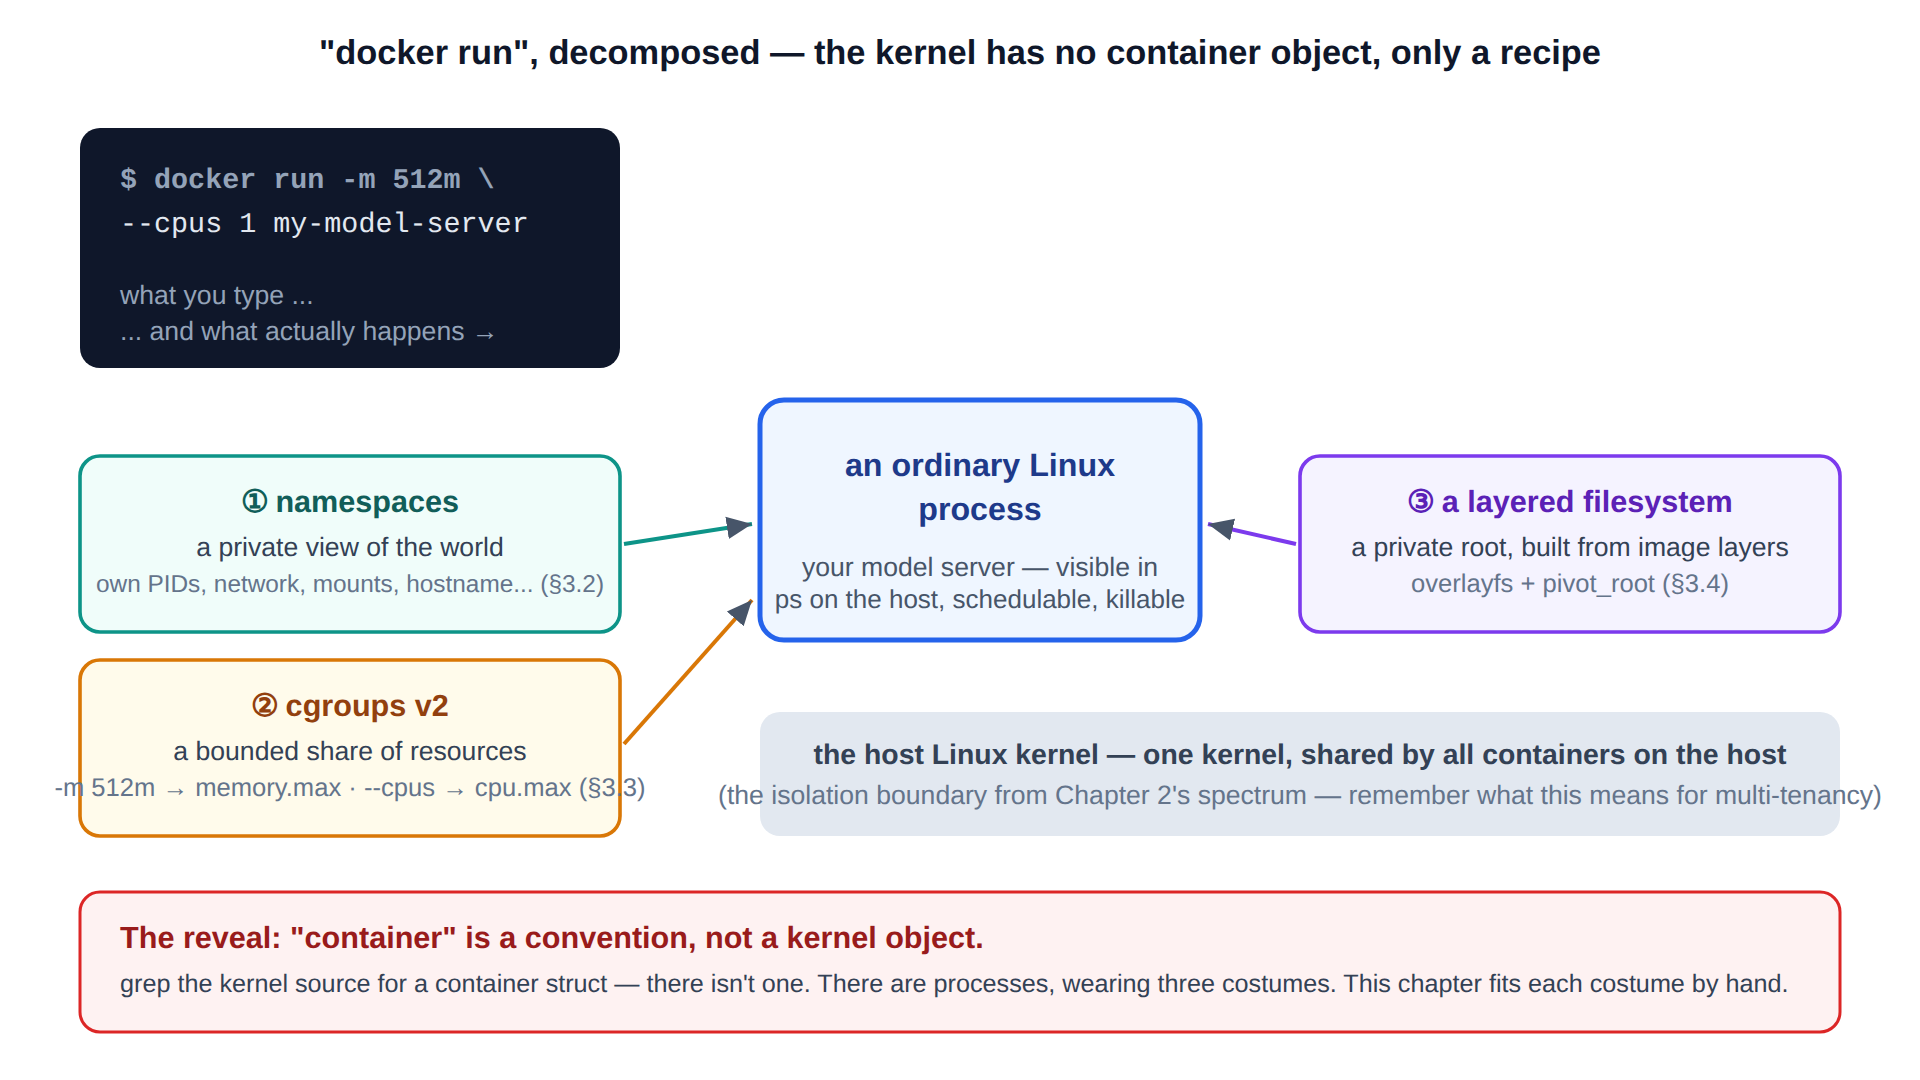
\includegraphics{figures/fig3-1_recipe.png}}\\[3pt]
  \figcaption{그림 3-1  docker run 분해하기. 컨테이너는 공유 커널 위의 일반 프로세스에 네임스페이스 + cgroup + 계층형 파일 시스템을 적용하는 레시피다.}
\end{tbbfigure}

\subsection*{직접 눈으로 확인하기}

이런 주장은 믿지 말고 확인해야 한다. Docker가 설치된 머신에서 컨테이너를 시작한 뒤 \textit{호스트에서} 심문해 보자. Docker 명령이 아니라 첫 운영체제 수업 때부터 써 온 평범한 프로세스 도구를 쓴다.

\begin{terminalbox}
\begin{Verbatim}[breaklines=true,breakanywhere=true,fontsize=\small,formatcom=\color{tbbtermfg},codes=\tbbcodeactive]
$ docker run -d --name demo -m 512m --cpus 1 python:3.11 sleep 9999
3f9a1c2b77e1...
$ docker inspect --format '{{.State.Pid}}' demo     # ask Docker for the host PID
41320
$ ps -o pid,ppid,rss,cmd -p 41320                  # plain ps, on the host
  PID   PPID   RSS  CMD
41320  41288  9184  sleep 9999
$ cat /proc/41320/cgroup                           # which budget group is it in?
0::/system.slice/docker-3f9a1c2b77e1....scope
$ cat /sys/fs/cgroup/system.slice/docker-3f9a*.scope/memory.max
536870912                                          # there is your -m 512m
$ ls -l /proc/41320/ns/pid                         # and its private view
... /proc/41320/ns/pid -> pid:[4026532871]
\end{Verbatim}
\end{terminalbox}
\figcaption{기록 3-1  일반 프로세스 도구를 사용해 호스트에서 실행 중인 컨테이너를 심문한 결과. cgroup과 네임스페이스가 연결된 프로세스(PID 41320)다.}

기록을 아래에서 위로 읽으면 다섯 줄에 이 장 전체가 예고되어 있다. 컨테이너는 \textbf{호스트 ps에 보인다}. 런타임 shim의 자식인 프로세스 41320이며, 다른 프로세스처럼 메모리 9 MB를 사용한다. \code{-m 512m} 플래그는 \textbf{파일 속 숫자}가 되었다(\code{memory.max = 536870912}, 3.3절). "격리"는 \code{/\allowbreak proc/\allowbreak 41320/\allowbreak ns/\allowbreak } 아래의 \textbf{네임스페이스 링크 집합}이다(3.2절). 호스트 커널은 이 프로세스를 스케줄링하고 사용량을 계산하며, 3.6절에서 생생히 보여 주듯 죽일 수도 있다. Docker의 기여는 설정을 오케스트레이션하는 것이지 새로운 종류의 무언가를 만들어 내는 것이 아니다.

\subsection*{신비를 벗기는 일이 중요한 이유(철학적인 이유만은 아니다)}

제2장의 격리 스펙트럼에서 이미 이 사실을 한 번 사용했다. 컨테이너가 호스트 커널을 공유하므로 멀티테넌트 플랫폼은 gVisor나 microVM을 선택한다. 그러나 레시피 관점은 이 책 내내 매주 운영 현장에서 값을 한다.

\begin{tbbitemize}
  \item \textbf{이 책의 나머지 동안 모델 서버는 컨테이너다.} 4주 차에는 이미지로 패키징하고, 5주 차에는 Kubernetes가 스케줄링하며, 9\textasciitilde{}12주 차에는 그 안에서 서빙한다. 자원 한도, 상태 검사, 네트워킹, GPU 접근 등 시스템이 컨테이너에 하는 모든 일은 결국 이 장의 세 메커니즘으로 귀결된다. 오작동하면 이 계층에서 디버깅한다.
  \item \textbf{이 장의 대미를 장식하는 것은 실전에서 가장 흔한 서빙 장애다.} \code{OOMKilled}, 종료 코드 137과 함께 애플리케이션 로그 없이 죽는 추론 pod도 memory.max가 cgroup 파일이고 OOM 킬러가 이를 강제한다는 사실을 알면 수수께끼가 아니다. 3.6절은 언젠가 오전 2시에 읽게 될 실제 \code{dmesg} 줄과 \code{kubectl} 출력을 통해 이 사고를 체크리스트로 바꾼다.
  \item \textbf{이미지 계층은 지연 시간 예산이다.} PyTorch/CUDA 이미지는 5–10 GB에 이른다. 새 노드로 이미지를 가져오는 시간이 12주 차 콜드 스타트 청구서에서 단일 항목으로는 최대일 때가 많다. \code{RUN rm}을 실행해도 아무것도 작아지지 않는 이유를 포함해 overlayfs(3.4절)를 이해하면 이미지 축소가 맹목적인 관습이 아니라 합리적인 작업이 된다.
  \item \textbf{디버깅의 성격이 바뀐다.} 컨테이너가 프로세스라는 사실을 알면 기록 3-1의 도구 상자를 어디서든 사용할 수 있다. \code{ps}, \code{/\allowbreak proc/\allowbreak <pid>/\allowbreak ns}, cgroup 파일, 내부로 들어가는 \code{nsenter}다. 상자가 더는 불투명하지 않고, "컨테이너에서는 작동합니다"가 대화의 끝이 아니게 된다.
\end{tbbitemize}

이 장의 구성은 레시피를 반영한다. 3.2\textasciitilde{}3.4절은 보는 것, 사용하는 것, 존재하는 것에 해당하는 재료를 하나씩 다루며, 각각 명령 기록과 계산 예시를 제시한다. 3.5절에서는 이번 주 시청 자료인 Liz Rice의 유명한 라이브 코딩 시연 구조를 따라 셸만으로 재료를 조립해 작동하는 컨테이너를 만든다. 3.6\textasciitilde{}3.7절에서는 이렇게 얻은 이해를 이 장에서 가장 가치 있는 운영 기술 하나에 쓴다. OOM 킬러를 예측하고 관찰하며 살아남는 법이다.

\begin{calloutbox}{tbbpurple}{tbbpurplefill}
{\normalsize\bfseries\color{tbbpurple}생각해 보기}\par\vspace{3pt}
\begin{tbbitemize}
  \item Docker for Mac/Windows는 내부에서 Linux VM을 실행한다. 이 절의 주장과 제2장을 이용해 왜 그래야 하는지 설명해 보자. 이 사실은 노트북 위에서 "컨테이너는 VM보다 가볍다"는 말에 어떤 함의를 갖는가?
  \item 기록 3-1에서 sleep의 부모는 입력한 docker CLI가 아니라 "shim" 프로세스(PID 41288)다. 수명이 긴 중간자가 유용한 이유를 추측해 보자. (힌트: Docker 데몬이 다시 시작되면 컨테이너에는 무슨 일이 일어나야 하는가?) 4주 차에 확인한다.
  \item 컨테이너가 그저 프로세스라면 \code{docker exec}는 무엇을 해야 하는가? 네임스페이스를 힌트 삼아 답을 그려 본 뒤, §3.2의 setns와 맞춰 보자.
\end{tbbitemize}
\end{calloutbox}

\section{네임스페이스: 세계를 보는 비공개 관점}

네임스페이스는 프로세스 테이블, 네트워크 스택, 마운트 테이블 같은 커널의 전역 자원 하나를 가져와 프로세스 그룹에 \textbf{그 관점의 비공개 사본}을 제공한다. 아무것도 에뮬레이션하지 않고 두 번째 커널도 나타나지 않는다(두 번째 커널을 띄우는 것은 제2장의 방식이었다). 커널은 네임스페이스마다 장부를 따로 관리하고 각 프로세스에 자신이 속한 장부를 보여 줄 뿐이다. PID 네임스페이스의 프로세스가 \code{getpid()}를 호출하면 커널은 호출자가 어느 네임스페이스에 속하는지 찾아 \textit{그곳에서 보이는} ID를 반환한다. 같은 커널과 같은 코드 경로지만 보는 사람마다 답이 다르다. 그림 3-2는 호스트와 컨테이너에 보이는 것을 비교하면서 고전적인 네임스페이스 여섯 개를 둘러본다.

\begin{tbbfigure}
  \adjustbox{max width=0.94\linewidth,max totalheight=0.46\textheight}{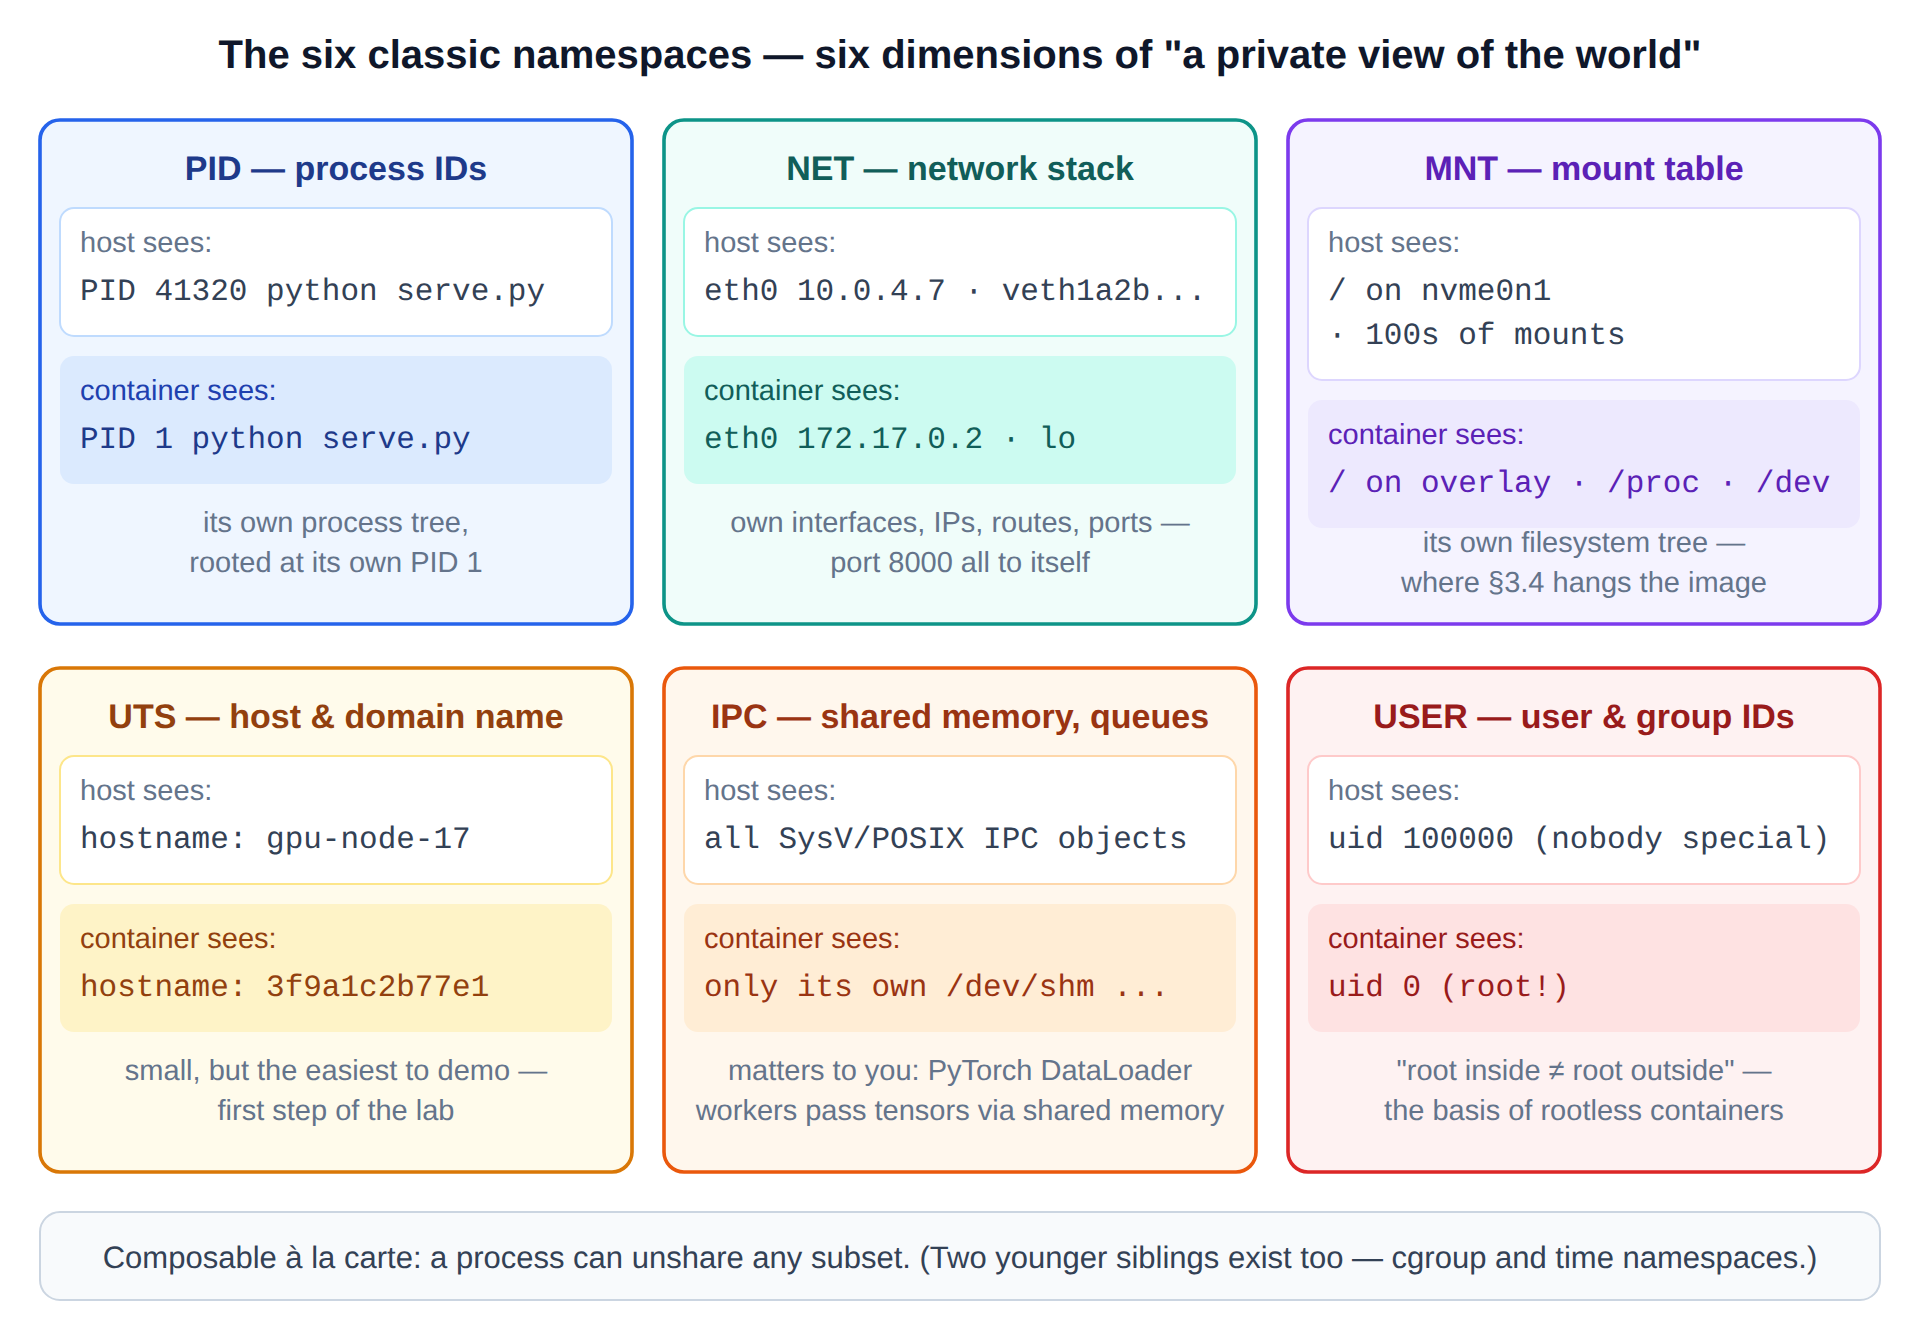
\includegraphics{figures/fig3-2_namespaces.png}}\\[3pt]
  \figcaption{그림 3-2  여섯 네임스페이스와 여섯 가지 비공개 차원: PID, 네트워크, 마운트, 호스트 이름, IPC, 사용자 ID. 원하는 것만 골라 조합할 수 있다.}
\end{tbbfigure}

\subsection*{API는 호출 세 개와 디렉터리 하나다}

그 결과에 비해 네임스페이스 API는 작다. \code{unshare()}는 \textit{호출한} 프로세스를 새로 만든 네임스페이스로 옮긴다. \code{unshare} 명령은 이를 감싸며 실습의 주력 도구다. \code{clone()}은 새 네임스페이스 안에 \textit{자식}을 바로 만들며 컨테이너 런타임이 사용한다. \code{setns()}는 핸들을 받아 기존 네임스페이스에 \textit{합류}한다. 3.1절의 예고에 답하므로 잠시 주목할 만하다. \code{docker exec}는 겉모습만 바꾼 \code{setns()}다. 대상 컨테이너의 네임스페이스 파일을 열고 합류한 뒤 그곳에서 셸을 실행한다. 마법의 문은 없다. 프로세스가 읽을 장부를 바꿀 뿐이다.

핸들은 검사할 수 있는 디렉터리에 있다. 모든 프로세스는 \code{/\allowbreak proc/\allowbreak <pid>/\allowbreak ns/\allowbreak }에 심볼릭 링크 형태로 네임스페이스 소속을 공개하며, 대괄호 속 숫자가 네임스페이스의 신원이다. \textbf{두 프로세스의 숫자가 같으면 같은 네임스페이스이고, 다르면 다른 네임스페이스다. 예외는 없다.}

\begin{terminalbox}
\begin{Verbatim}[breaklines=true,breakanywhere=true,fontsize=\small,formatcom=\color{tbbtermfg},codes=\tbbcodeactive]
$ ls -l /proc/self/ns/            # my shell, on the host
mnt -> mnt:[4026531841]   net -> net:[4026531840]
pid -> pid:[4026531836]   uts -> uts:[4026531838]  ...
$ ls -l /proc/41320/ns/           # the container process from Transcript 3-1
mnt -> mnt:[4026532868]   net -> net:[4026532866]
pid -> pid:[4026532871]   uts -> uts:[4026532864]  ...
# every number differs -> different views on every axis.
# same number would mean: shared namespace. Free debugging test.
\end{Verbatim}
\end{terminalbox}
\figcaption{기록 3-2  네임스페이스 신원은 검사할 수 있다. inode 번호가 같으면 네임스페이스를 공유한다. "컨테이너에서 X가 보이지 않는다"면 가장 먼저 확인할 항목이다.}

네임스페이스는 원하는 것만 골라 조합할 수 있다. 프로세스가 NET만 분리할 수도 있고(네트워크 테스트에서 흔하다), 모든 것을 한꺼번에 분리할 수도 있다(컨테이너). 더 늦게 등장한 cgroup 네임스페이스와 시간 네임스페이스까지 더하면 현대의 여덟 개가 되지만, 이 장은 고전적인 여섯 개를 다룬다.

\subsection*{PID: 프로세스 하나, 두 가지 진실}

PID 네임스페이스는 컨테이너에 자체 PID 1을 뿌리로 하는 프로세스 트리를 제공한다(그림 3-3 왼쪽). 따라서 같은 커널 태스크가 호스트에는 PID 41320, 자신에게는 PID 1이라는 두 신원을 갖는다. 두 번째 신원이 생기는 모습을 직접 볼 수 있다.

\begin{terminalbox}
\begin{Verbatim}[breaklines=true,breakanywhere=true,fontsize=\small,formatcom=\color{tbbtermfg},codes=\tbbcodeactive]
$ sudo unshare --pid --fork --mount-proc bash    # new PID ns + fresh /proc
$ echo $$                                        # "what is my PID?"
1
$ ps aux
USER  PID  %CPU  %MEM  ... CMD
root    1   0.0   0.0  ... bash
root    8   0.0   0.0  ... ps aux
# two processes exist in this whole "machine" - and I am init.
\end{Verbatim}
\end{terminalbox}
\figcaption{기록 3-3  새 PID 네임스페이스 내부. 셸은 PID 1이고 프로세스 테이블에는 항목 두 개가 있다. (--fork가 중요하다. PID 소속은 자식에게 적용되므로 unshare가 셸을 새 세계로 fork해야 한다.)}

\code{--mount-proc} 플래그가 함께 따라오는 이유는 무엇인가? \code{ps}는 커널에 직접 묻지 않고 \textit{/proc 파일 시스템을 읽는다}. \code{/\allowbreak proc}가 여전히 호스트의 마운트를 보여 주면 새 네임스페이스 안에서도 \code{ps}는 호스트의 수천 개 프로세스를 거리낌 없이 보고한다. \code{/\allowbreak proc}를 다시 마운트하면 도구가 새로운 진실을 말한다. 조금 철학적인 이 교훈을 기억하자. \textbf{Linux 시스템에 대한 관점은 마운트가 정직한 만큼만 정직하다.} 실습의 4단계와 14주 차 모니터링 각주에서 다시 등장한다.

\subsection*{PID 1은 숫자가 아니라 직무다}

Unix는 PID 1(init)에 의무 두 가지를 부여한다. 대부분의 애플리케이션 코드는 이를 생각해 볼 일이 없다 — 컨테이너에 담겨 갑자기 \textit{자신이} PID 1이 되기 전까지는. 첫째는 \textbf{신호}다. PID 1에 대해 커널은 보통 SIGTERM을 치명적으로 만드는 기본 핸들러를 비활성화한다. 명시적인 SIGTERM 핸들러가 없는 프로세스가 PID 1로 실행되면 SIGTERM을 그냥 \textit{무시한다}. 둘째는 \textbf{회수}다. 프로세스가 죽으면 부모가 \code{wait()}를 호출해 종료 상태를 수집해야 한다. 그때까지 프로세스 테이블에 죽은 항목인 \textbf{좀비}로 남는다. 고아 프로세스는 PID 1에 다시 연결되므로, PID 1은 다른 프로세스의 자식을 영원히 회수해야 한다. 그렇지 않으면 \code{pids.max}나 노드가 질식할 때까지 좀비가 쌓인다.

이 두 의무를 무시하는 모델 서버에서 Kubernetes 롤링 배포(13주 차)가 어떻게 흘러가는지 돌려 보자. t=0에 kubelet이 컨테이너의 PID 1, 즉 핸들러를 설치하지 않은 Python 서버에 SIGTERM을 보낸다. 아무 일도 일어나지 않고, 서버는 끝내지 못할 요청을 계속 받는다. 기본 유예 기간인 t=30 s가 되면 kubelet이 인내심을 잃고 SIGKILL을 보낸다. 서버는 요청 처리 중간에 죽고, 처리 중인 모든 요청이 오류를 낸다. 이 과정이 \textbf{모든 배포마다} 반복된다. 스스로 만들어 낸 영구 장애 제조기인데, 겉보기에는 "K8s가 불안정하다"로 보인다. 해결책은 작고 표준적이다.

\begin{tbbitemize}
  \item \textbf{서버에서 SIGTERM을 처리한다.} 새 요청을 받지 않고, 처리 중인 요청을 비운 뒤 종료한다. FastAPI/uvicorn과 대부분의 제대로 된 서버는 신호를 받기만 하면 이 작업을 한다. 다음 항목을 보자.
  \item \textbf{신호가 서버에 도달하는지 확인한다.} 고전적인 Dockerfile 버그가 있다. \textit{셸 형식}의 \code{CMD python serve.py}는 \code{/\allowbreak bin/\allowbreak sh -c "python serve.py"}를 실행한다. 셸이 PID 1이며 자식에게 SIGTERM을 전달하지 않는다. exec 형식(\code{CMD ["python", "serve.py"]})을 사용해 서버 \textit{자체가} PID 1이 되고 실제 신호를 받게 한다.
  \item \textbf{또는 진짜 init을 설치한다.} \code{tini}(플래그 하나: \code{docker run --init})는 신호를 전달하고 좀비를 회수하는 수백 줄짜리 PID 1이다. 애플리케이션이 다시 평범한 자식이 될 수 있다.
\end{tbbitemize}

\begin{tbbfigure}
  \adjustbox{max width=0.94\linewidth,max totalheight=0.46\textheight}{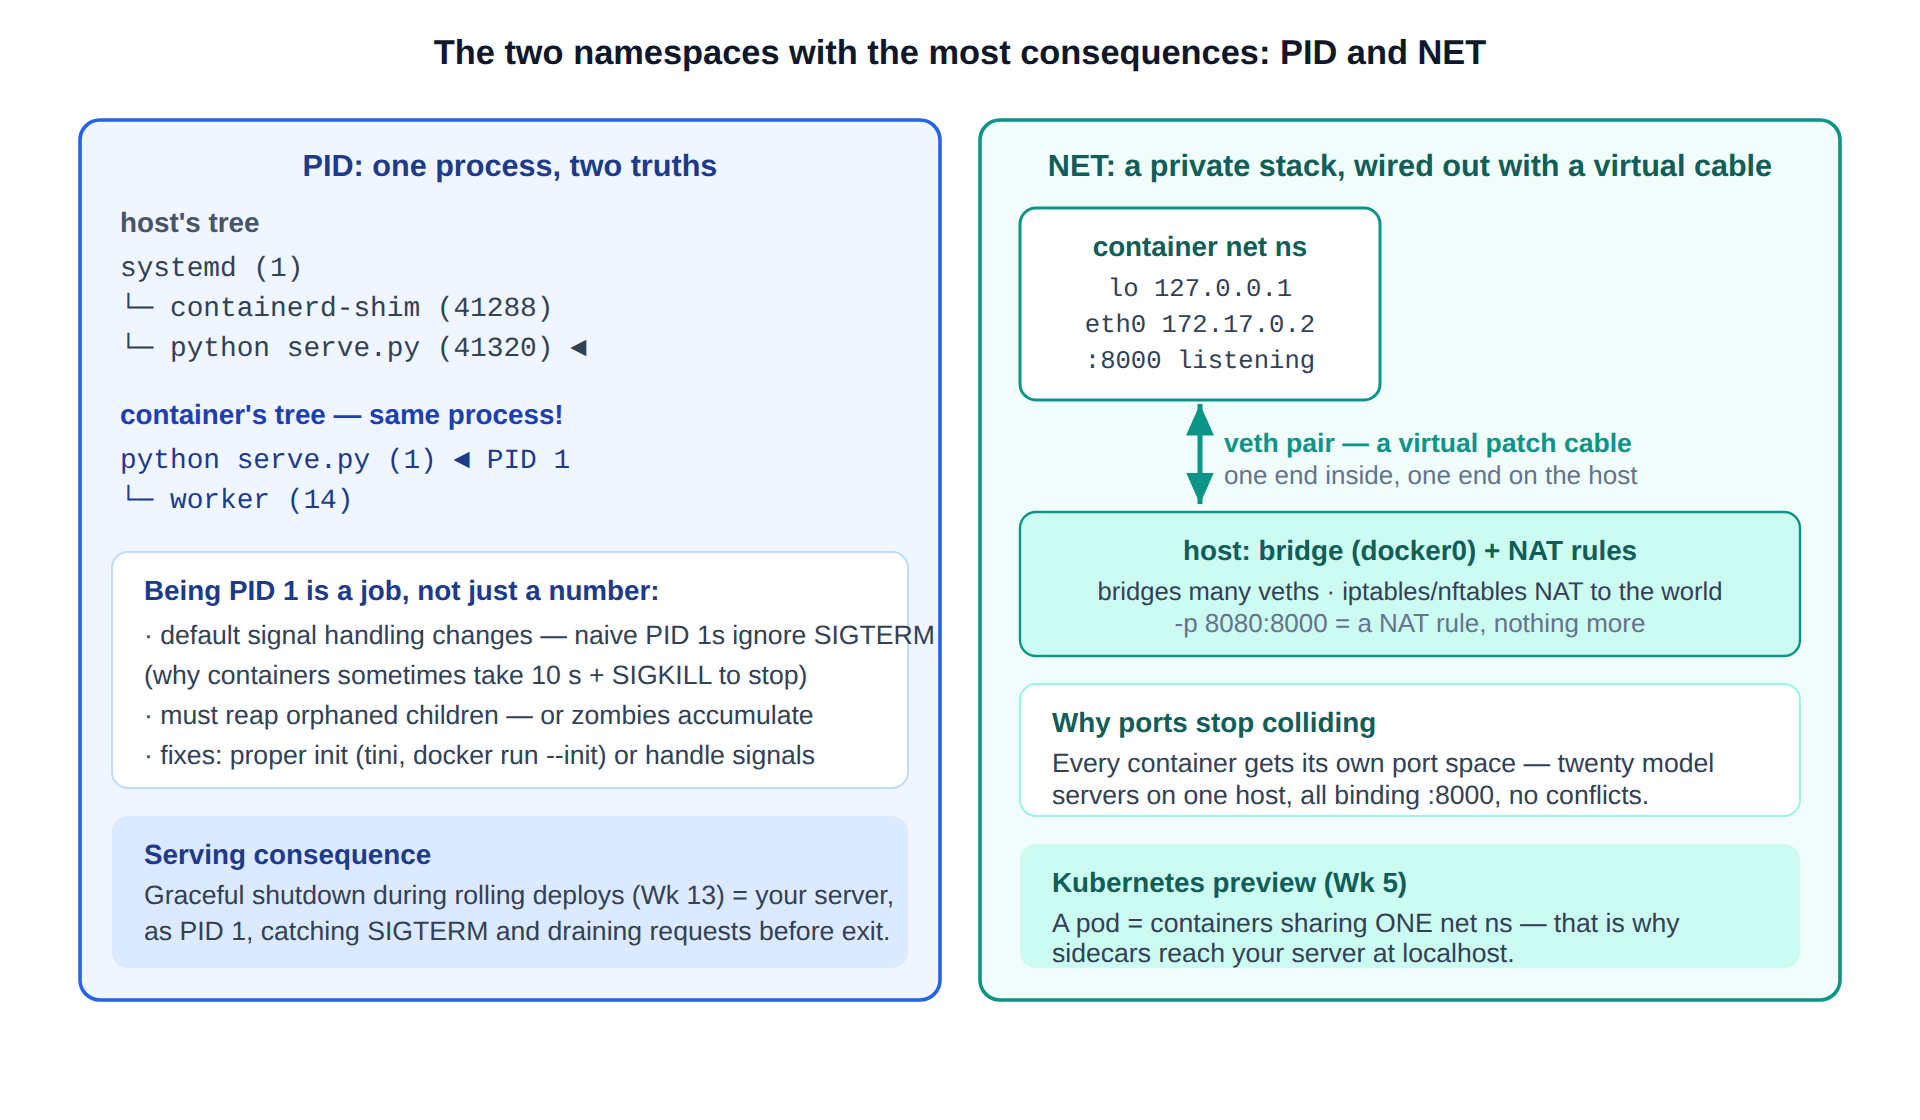
\includegraphics{figures/fig3-3_pidnet.png}}\\[3pt]
  \figcaption{그림 3-3  중요한 결과를 만드는 두 네임스페이스. 왼쪽 PID는 프로세스 하나의 두 신원과 PID 1의 의무를 보여 준다. 오른쪽 NET은 veth 쌍을 통해 호스트 브리지에 연결된 비공개 스택이다.}
\end{tbbfigure}

\subsection*{NET: 비공개 스택과 요청 하나의 생애}

NET 네임스페이스는 여섯 개 중 가장 물리적으로 느껴진다. 컨테이너가 인터페이스, IP 주소, 라우팅 테이블, 방화벽 규칙, 그리고 무엇보다 \textbf{자체 포트 공간}을 포함한 완전한 비공개 네트워크 스택을 얻는다. 호스트 하나의 모델 서버 레플리카 20개가 충돌 없이 모두 \code{:8000}에 바인딩할 수 있다. 이 덕분에 레플리카 서버군을 관리할 수 있다. 1998년처럼 포트를 하나씩 배정할 필요가 없다.

갓 만든 비공개 스택은 아직 \textit{아무 데도 연결되지 않은} 스택이기도 하다. 새 NET 네임스페이스에는 루프백 장치만 있고 그마저 내려가 있다. 표준 배선(그림 3-3 오른쪽)은 패치 케이블처럼 연결한 가상 NIC 두 개, 즉 \textbf{veth 쌍}을 만든다. 제2장의 virtio 정신을 네트워킹에 적용한 것이다. 한쪽 끝은 컨테이너 안에 두고 \code{eth0}으로 이름을 바꾸며, 다른 끝은 호스트의 소프트웨어 \textbf{브리지}(Docker의 \code{docker0})에 연결한다. 구체적으로, 노트북에서 출발한 요청 하나가 \code{-p 8080:8000}으로 공개된 컨테이너의 8000번 포트에 닿기까지를 따라가 보자.

\begin{tbbitemize}
  \item \textbf{도착:} \code{host:8080}으로 주소가 지정된 패킷이 호스트의 실제 NIC에 도착한다.
  \item \textbf{변환:} \code{-p 8080:8000}을 지정할 때 Docker가 설치한 iptables/nftables DNAT 규칙이 목적지를 \code{172.17.0.2:8000}으로 고쳐 쓴다. \textit{공개한 포트는 문자 그대로 NAT 규칙 하나다.}
  \item \textbf{브리지와 통과:} 호스트가 패킷을 \code{docker0}으로 라우팅하고, 브리지가 컨테이너의 veth로 전달한다. 패킷은 NET 네임스페이스 안의 \code{eth0}에 나타나며 서버가 \code{:8000}에서 수신 대기한다.
  \item \textbf{반환:} 응답은 경로를 거슬러 간다. 연결 추적이 소스의 NAT를 되돌리므로 노트북은 아무것도 모른 채 \code{host:8080}의 응답을 본다.
\end{tbbitemize}

5주 차를 위해 미리 기록해 둘 내용이 있다. Kubernetes \textbf{pod}는 하나의 NET 네임스페이스를 소유하는 작은 "pause" 자리 표시자 프로세스를 통해 \textbf{NET 네임스페이스 하나를 공유하는} 컨테이너로 정의된다. 이 한 가지 설계 결정 때문에 사이드카(sidecar) 프록시가 \code{localhost}로 모델 서버에 도달하고, "pod당 IP 하나"가 가능하며, pod 안의 컨테이너 둘은 포트가 충돌할 \textit{수 있지만} pod 둘은 충돌하지 않는다.

\subsection*{USER: 내부의 root는 외부의 root가 아니다}

USER 네임스페이스는 명시적인 테이블 \code{/\allowbreak proc/\allowbreak <pid>/\allowbreak uid\_map}으로 사용자 ID를 다시 매핑한다. \code{0 100000 65536}이라는 매핑은 "이 네임스페이스 내부의 uid 0이 외부의 uid 100000에 대응하며 65536개 ID 범위에 적용된다"는 뜻이다. 따라서 프로세스는 내부에서 비공개 파일 시스템에 패키지를 설치하고 비공개 80번 포트에 바인딩하는 \textit{root}이면서, 호스트 커널에는 특권 없는 uid 100000일 수 있다. 내부에서 파일을 만들면 호스트에서는 특별할 것 없는 100000이 소유한다. 이것이 \textbf{루트리스 컨테이너(rootless container)}(Podman의 대표 기능, Docker의 루트리스 모드)의 기반이다. 런타임까지 특권 없이 실행하여 컨테이너 탈출의 결과를 크게 줄인다. 루트리스 컨테이너를 탈출한 공격자는 호스트에서 아무 권한 없는 사용자로 나온다. (완화책일 뿐 제2장의 microVM 경계는 아니다. 공유 커널의 시스템 호출 표면이 남아 있다.)

\subsection*{UTS와 IPC: 짧지만 가볍지 않게}

UTS(자체 호스트 이름)는 가장 작지만 가장 많이 가르쳐 주는 네임스페이스다. 내부 호스트 이름을 바꾸면서 호스트가 그대로인 모습을 보는 것은 관점이 실제로 갈라졌음을 입증하는 가장 빠른 방법이며, 그래서 실습 2단계에 둔다. IPC는 System V와 POSIX 공유 메모리를 비공개로 만든다. 호랑이 담배 피우던 시절의 각주처럼 들리지만 \textbf{PyTorch DataLoader 워커가 `/dev/shm`에 마운트된 공유 메모리를 통해 프로세스 사이에서 텐서를 전달한다}는 사실을 떠올리면 달라진다. Docker의 기본 \code{/\allowbreak dev/\allowbreak shm}은 64 MB다. 워커가 여러 개인 DataLoader가 실제 배치를 처음 옮기면 이 상한에 부딪혀, 아무 도움도 안 되기로 악명 높은 \code{ERROR: Unexpected bus error encountered in worker. This might be caused by insufficient shared memory (shm)}와 함께 죽는다. 모든 ML 엔지니어가 결국 외우는 해결책은 \code{--shm-size=8g}(또는 K8s의 동등한 볼륨)이다. 이제 그 플래그가 어느 네임스페이스를 향한 것인지 안다.

\begin{calloutbox}{tbbpurple}{tbbpurplefill}
{\normalsize\bfseries\color{tbbpurple}생각해 보기}\par\vspace{3pt}
\begin{tbbitemize}
  \item Kubernetes pod 하나에 컨테이너 두 개가 있다. 그림 3-2의 여섯 축을 사용해 어느 네임스페이스를 공유하고 어느 것을 비공개로 유지하는지 생각해 보자. (localhost로 통신하지만 파일 시스템은 다르다는 점에서 추론할 수 있다.)
  \item 로컬 테스트(python serve.py, Ctrl-C 작동)에서는 서버가 SIGTERM을 잘 처리하지만 컨테이너에서는 무시한다. 이 절을 이용해 가장 가능성 높은 원인 두 가지와 각각의 한 줄 해결책을 제시하라.
  \item USER 네임스페이스 안에서 uid 0으로 실행하는 것이 네임스페이스 없이 uid 0으로 실행하는 것보다 훨씬 안전하지만, 제2장의 microVM 경계만큼 강하지는 않은 이유는 무엇인가? 남아 있는 공유 표면의 이름을 쓰라.
\end{tbbitemize}
\end{calloutbox}

\section{cgroups v2: 머신의 제한된 몫}

네임스페이스는 프로세스에 보이는 것을 바꾸지만 소비할 수 있는 양은 제한하지 않는다. 아름답게 비공개인 PID 트리를 가진 컨테이너화된 모델 서버도 노드의 모든 코어와 RAM을 마지막 바이트까지 먹어 치우고 이웃 레플리카 19개를 함께 쓰러뜨릴 수 있다. 두 번째 재료인 \textbf{컨트롤 그룹, cgroups v2}는 예산 시스템이다. 프로세스를 그룹에 넣고 그룹별 \textbf{컨트롤러}가 CPU, 메모리, I/O, 프로세스 수를 계량하고 제한한다. 네임스페이스가 "어떤 세계가 보이는가?"에 답한다면 cgroup은 "머신을 얼마만큼 사용할 수 있는가?"에 답한다(그림 3-4).

\begin{tbbfigure}
  \adjustbox{max width=0.94\linewidth,max totalheight=0.46\textheight}{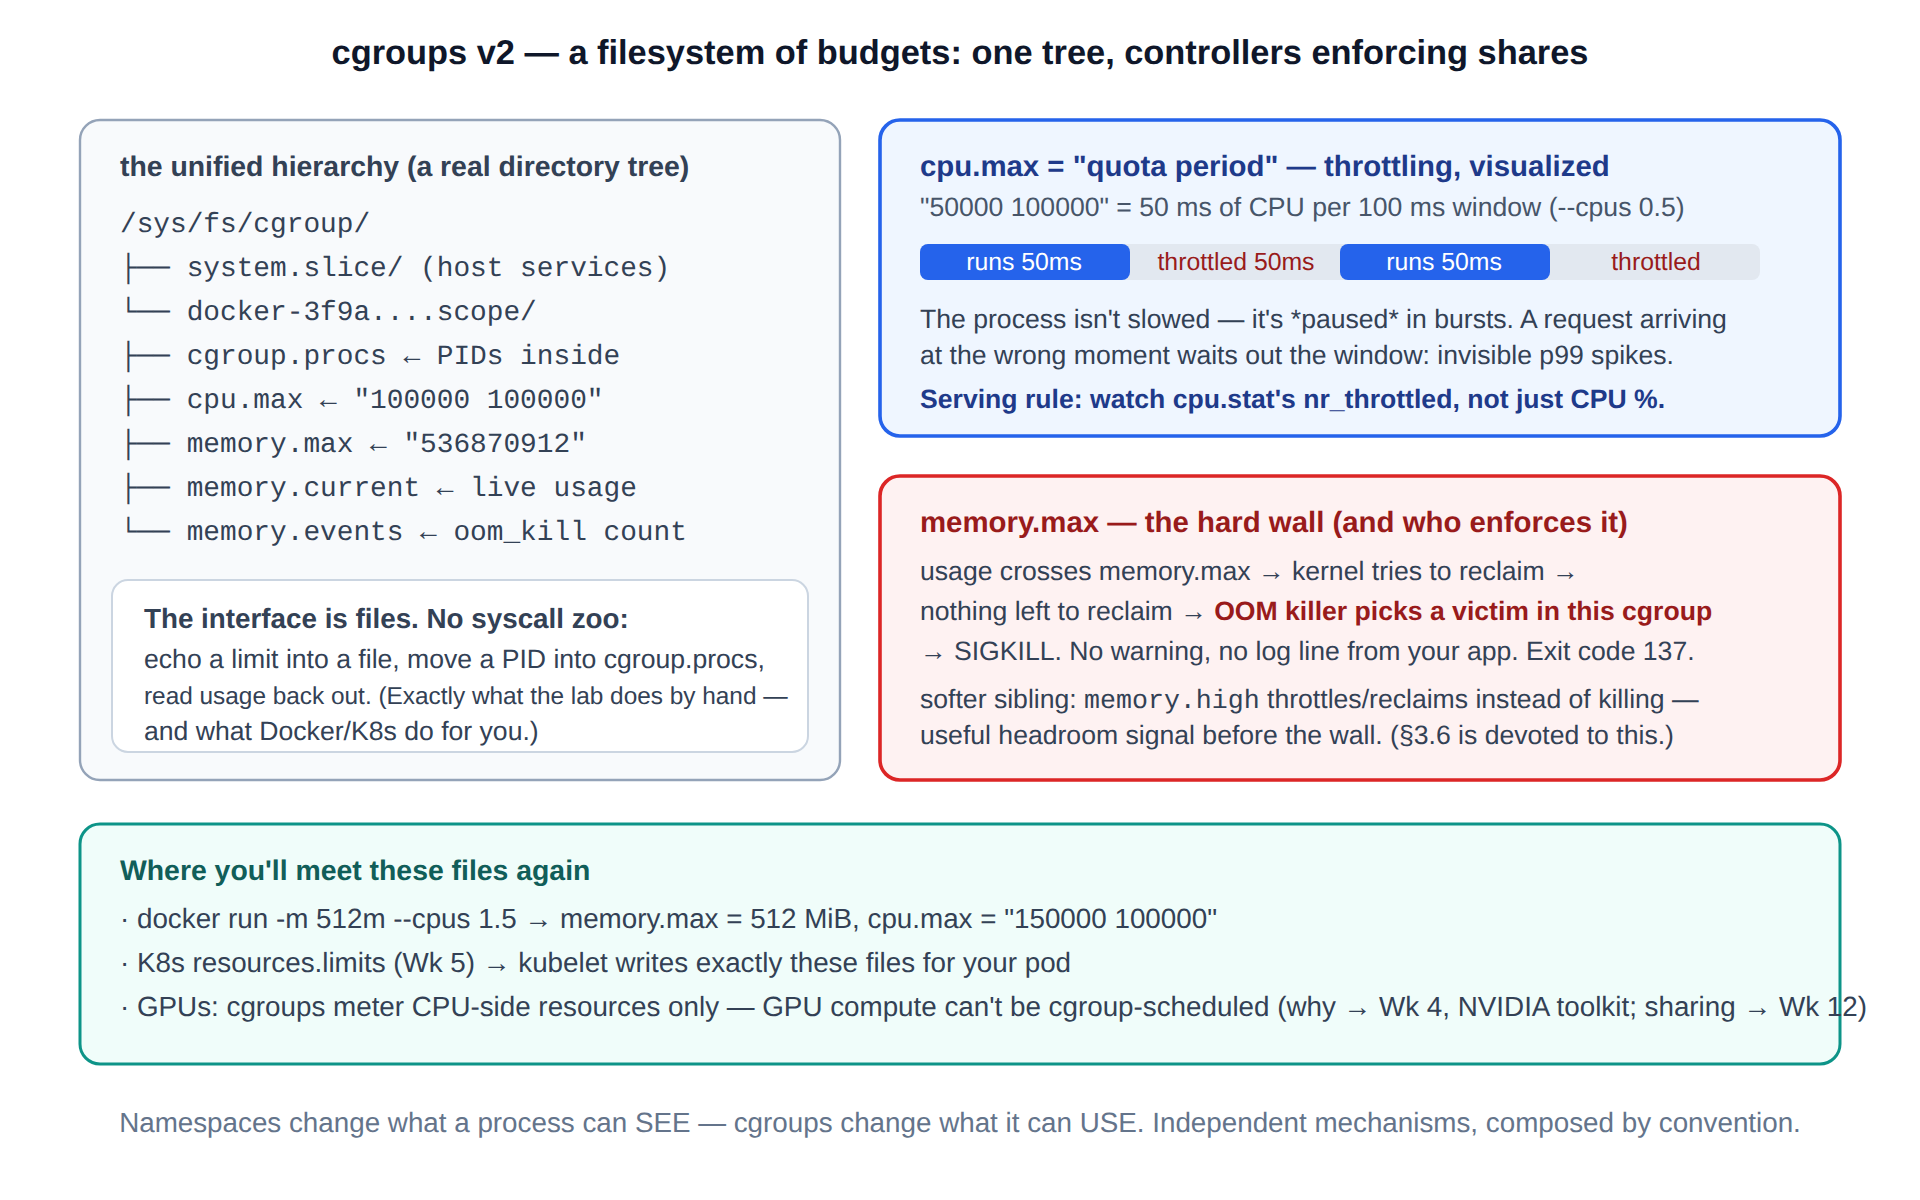
\includegraphics{figures/fig3-4_cgroups.png}}\\[3pt]
  \figcaption{그림 3-4  cgroups v2는 파일 시스템으로 공개된 단일 계층이다. cpu.max는 뭉텅이로 스로틀링해 p99를 위협하며, memory.max는 OOM 킬러가 강제하는 단단한 벽이다.}
\end{tbbfigure}

\subsection*{인터페이스는 파일 시스템이다 — 라이브러리가 필요 없다}

cgroups v2는 \code{/\allowbreak sys/\allowbreak fs/\allowbreak cgroup} 아래에 통합 트리 하나를 제공하며, 전체 API가 파일 작업이다. 완전한 예산을 만들고 적용한 뒤 다시 읽는 과정을 살펴보자. 실습 5단계의 예고이기도 하다.

\begin{terminalbox}
\begin{Verbatim}[breaklines=true,breakanywhere=true,fontsize=\small,formatcom=\color{tbbtermfg},codes=\tbbcodeactive]
$ cd /sys/fs/cgroup && sudo mkdir demo        # a new group = a new directory
$ echo "50000 100000" | sudo tee demo/cpu.max # 50ms CPU per 100ms window (0.5 CPU)
$ echo $((256*1024*1024)) | sudo tee demo/memory.max   # 256 MiB hard wall
$ echo $$ | sudo tee demo/cgroup.procs        # enroll THIS shell (children follow)
$ cat demo/memory.current                     # live usage, in bytes
3862528
$ cat demo/cpu.stat | head -4
usage_usec 184220
user_usec  132009
system_usec 52211
nr_throttled 0                                # (watch this one in a moment)
\end{Verbatim}
\end{terminalbox}
\figcaption{기록 3-4  다섯 번의 파일 작업으로 만든 완전한 cgroup 예산. mkdir, 한도를 쓰는 echo 두 번, 등록하는 echo 한 번, 관찰하는 cat이다. Docker와 kubelet이 사용자를 대신해 정확히 이 일을 한다.}

\code{mkdir}, \code{echo}, \code{cat}이 메커니즘의 전부다. 대필자를 알아보자(아래 표 3-2). Docker 플래그나 Kubernetes 한도는 결국 프로그램이 이 파일에 숫자를 쓰는 것이다. v2의 단일 트리는 v1의 컨트롤러별로 뒤얽힌 계층을 대체했다. 현대 배포판과 Kubernetes는 v2를 기본으로 사용하며 이 책도 줄곧 v2를 다룬다.

\begin{tbbtablewrap}
  \begin{tabular}{@{}>{\raggedright\arraybackslash}m{\dimexpr 0.2447\tbltextwidth-2\tabcolsep\relax} >{\raggedright\arraybackslash}m{\dimexpr 0.4574\tbltextwidth-2\tabcolsep\relax} >{\raggedright\arraybackslash}m{\dimexpr 0.2979\tbltextwidth-2\tabcolsep\relax}@{}}
  \arrayrulecolor{tbbnavy}\specialrule{1pt}{0pt}{0pt}
  \rowcolor{tbbtablehead}{\centering \bfseries\color{tbbnavy}파일} & {\centering \bfseries\color{tbbnavy}의미} & {\centering \bfseries\color{tbbnavy}일반적인 작성자} \\
  \arrayrulecolor{tbbnavy}\specialrule{0.7pt}{0pt}{2pt}
  {\textbf{cgroup.procs}} & {이 그룹에 등록한 PID(프로세스를 옮기려면 씀)} & {런타임 / 사용자(실습)} \\
  \arrayrulecolor{tbbtableborder}\hline
  {\textbf{cpu.max}} & {하드 할당량: µs 단위 "<quota> <period>", 예: "50000 100000" = 0.5 CPU} & {docker --cpus, kubelet(한도)} \\
  \arrayrulecolor{tbbtableborder}\hline
  {\textbf{cpu.weight}} & {경합 시 비례 몫(1–10000), 소프트하고 남는 자원을 활용함} & {kubelet(요청량에서 계산)} \\
  \arrayrulecolor{tbbtableborder}\hline
  {\textbf{cpu.stat}} & {사용량 + nr\_throttled / throttled\_usec — 스로틀링(throttling) 진단} & {(읽기 전용 텔레메트리)} \\
  \arrayrulecolor{tbbtableborder}\hline
  {\textbf{memory.max}} & {단단한 메모리 벽(memory wall), 회수 실패 후 초과 → OOM 강제 종료} & {docker -m, kubelet(한도)} \\
  \arrayrulecolor{tbbtableborder}\hline
  {\textbf{memory.high}} & {소프트 상한: 스로틀링 + 회수, 강제 종료 없음 — 경보선(§3.6)} & {사용자 / 플랫폼 정책} \\
  \arrayrulecolor{tbbtableborder}\hline
  {\textbf{memory.current}} & {그룹의 실시간 사용량 — 실습에서 관찰} & {(읽기 전용 텔레메트리)} \\
  \arrayrulecolor{tbbtableborder}\hline
  {\textbf{memory.events}} & {oom\_kill을 포함한 카운터(counter) — OOM 증거 장부} & {(읽기 전용 텔레메트리)} \\
  \arrayrulecolor{tbbtableborder}\hline
  {\textbf{pids.max}} & {최대 프로세스/스레드 수 — 포크 폭탄 울타리} & {docker --pids-limit} \\
  \arrayrulecolor{tbbnavy}\specialrule{1pt}{2pt}{0pt}
  \end{tabular}\par
  \figcaption{표 3-1  실제로 다룰 cgroup v2 파일}
\end{tbbtablewrap}

\subsection*{CPU: 할당량은 뭉텅이로 스로틀링한다 — 지연 시간 계산 예시}

CPU 컨트롤러에는 성격이 \textit{매우} 다른 조절 장치 두 개가 있다. \code{cpu.weight}는 \textbf{경합할 때만} CPU를 비례 배분한다. 바쁜 4코어 머신에서 가중치 300 대 100이면 대략 코어 3개 대 1개를 얻지만, 이웃이 쉬면 어느 그룹이든 전부 사용할 수 있다. 노는 자원을 놀리지 않는 방식이며, 이를 강제하느라 사이클을 낭비하는 일도 없다. \code{cpu.max}는 주기가 있는 하드 할당량이다. \code{"50000 100000"}은 이웃이 쉬든 말든 \textit{100 ms 창마다 이 그룹이 50 ms 동안 실행될 수 있다}는 뜻이다. 강제 방식이 중요한 미묘함이다. 부드럽게 2× 느려지는 것이 아니라 \textbf{스로틀링}한다. 그룹은 창의 할당량을 소진할 때까지 제 속도 그대로 내달리다가, 다음 창이 열릴 때까지 멈춘다.

산술로 체감해 보자. 추론 요청 하나에 \textbf{CPU 시간 30 ms}가 필요하고 컨테이너 할당량이 \code{"20000 100000"}이라고 하자. 실제 클러스터가 "소형" 서비스에 설정하는 0.2 CPU다. 최선의 경우에는 새 창이 시작될 때 요청이 도착한다. 20 ms 동안 실행하고 할당량에 도달해 \textbf{80 ms 동안 멈춘} 뒤 다음 창에서 마지막 10 ms를 실행한다. 완료까지 \textbf{110 ms}가 걸리며 그중 80 ms는 강제 일시 중지다. 최악의 경우에는 앞선 요청이 할당량을 막 소진한 뒤 도착한다. 실행을 시작하기도 전에 최대 80 ms를 더 기다려 CPU 작업 30 ms에 \textbf{190 ms} 가까이 걸린다. 한편 부하가 적은 p50 요청은 창 하나 안에 완전히 들어가 아무 영향도 받지 않을 수 있다. 특유의 징후는 \textbf{p50은 멀쩡한데 p99는 창 잔여 시간의 대략 배수 단위로 뾰족하게 튀고, 애플리케이션 프로파일러에는 아무것도 보이지 않는다}는 것이다. 프로세스가 실행되지 않았으므로 프로파일링할 것도 없다.

\begin{terminalbox}
\begin{Verbatim}[breaklines=true,breakanywhere=true,fontsize=\small,formatcom=\color{tbbtermfg},codes=\tbbcodeactive]
# after driving load through the throttled cgroup from Transcript 3-4:
$ cat demo/cpu.stat
usage_usec     9184220
nr_periods     412
nr_throttled   118        # windows in which we hit the quota
throttled_usec 8221340    # 8.2 s of enforced pause, total
\end{Verbatim}
\end{terminalbox}
\figcaption{기록 3-5  스로틀링 진단. 부하가 걸릴 때 nr\_throttled가 증가하면 p99 급증은 코드가 아니라 여기서 만들어진다.}

표준 해결책은 메커니즘에서 바로 나온다. 할당량을 높이거나, 지연 시간이 중요한 pod에서는 하드 상한보다 \textbf{가중치}(요청량)를 선호해 유휴 용량을 계속 사용할 수 있게 한다. 또는 플랫폼이 무엇을 설정하는지 이해하고 실질적인 일시 중지를 줄인다. 5주 차에는 이 절을 근거로 "K8s CPU 한도를 설정해야 하는가?"라는 논쟁에 돌아온다. 이 이야기는 제2장의 스틸 타임과 나란히 기억해 두자. \textbf{서로 다른 두 메커니즘이 주는 교훈은 하나다. 코드 아래 계층이 꼬리 지연 시간을 만들어 낼 수 있다.}

\subsection*{메모리: 집행자가 지키는 단단한 벽 — 메모리 회수의 미묘함}

메모리 컨트롤러의 \code{memory.max}는 진정한 하드 한도지만, 벽에 이르는 길에는 순진한 그림이 놓치는 중간 단계가 하나 있다. \textbf{메모리 회수}다. 그룹 사용량이 한도에 도달하면 커널은 먼저 다시 만들 수 있는 메모리를 해제하려 한다. 대표적으로 RAM에 캐시한 파일 내용인 \textbf{페이지 캐시(page cache)}가 있다. 대시보드를 읽을 때 중요하다. \code{memory.current}는 페이지 캐시를 포함하므로, 대형 파일을 스트리밍하는 컨테이너(예: 모델 가중치 로딩)가 몇 시간 동안 한도에 붙어 있는 \textit{것처럼 보여도} 완벽하게 건강할 수 있다. 캐시는 회수 가능한 짐이지 필수 메모리가 아니다. 회수할 수 없는 것은 Python 힙과 텐서 같은 \textbf{익명 메모리}다. 벽에 닿은 사용량이 익명 메모리라면 회수에 실패하고, 커널은 \textbf{이 cgroup 범위의 OOM 킬러}를 호출한다. 그룹에서 가장 큰 프로세스(\code{oom\_score\_adj}로 조정 가능)를 골라 항소할 수도 잡을 수도 없고 피해자에게 보이지도 않는 SIGKILL을 보낸다. 애플리케이션 로그에는 아무것도 없고 셸에는 \textbf{종료 코드 137}(128 + 9)이 보이며 Kubernetes는 \code{OOMKilled}를 찍는다. 더 온화한 형제인 \code{memory.high}는 죽이지 \textit{않고} 스로틀링하고 공격적으로 회수한다. 3.6절에서 설정할 경보선이며, 여기서부터의 자세한 이야기는 그 절이 도맡는다.

\subsection*{cgroup이 심판 볼 수 있는 것과 없는 것}

나머지 컨트롤러도 살펴보자. \code{io}는 블록 장치 대역폭과 IOPS를 계량하며, 가중치 로딩이 공유 디스크를 두들길 때 중요하다. \code{pids}는 프로세스 수를 제한하는 Liz Rice 시연의 포크 폭탄 울타리다. \code{cpuset}은 그룹을 특정 코어에 고정하며, 제2장 전용 코어 인스턴스의 컨테이너 사촌이다. 이 책의 방향을 결정하므로 없는 것에도 주목해야 한다. \textbf{cgroup에는 GPU 컨트롤러가 없다.} 커널은 \code{/\allowbreak dev/\allowbreak nvidia*} 장치에 대한 \textit{접근}을 통제할 수 있으며, 권한 수준에서 \code{--gpus}가 작동하는 방식이다. 4주 차에 툴킷의 내부 배관을 들여다본다. 그러나 cgroup 트리에는 \code{cpu.max}와 \code{memory.max}처럼 GPU 계산 시간을 나누거나 VRAM을 분할하는 것이 없다. 구체적으로 GPU 하나에 프로세스 둘을 놓으면 어느 쪽이든 VRAM 전체를 \code{cudaMalloc}하거나 SM을 독점할 수 있다. 이 부재 때문에 GPU 공유에는 제2장의 공급자 메커니즘인 시간 분할, MPS, MIG가 필요하며 12주 차 GPU 공유 도구 상자는 이 절과 전혀 다르게 생겼다.

\begin{tbbtablewrap}
  \begin{tabular}{@{}>{\raggedright\arraybackslash}m{\dimexpr 0.3511\tbltextwidth-2\tabcolsep\relax} >{\raggedright\arraybackslash}m{\dimexpr 0.3298\tbltextwidth-2\tabcolsep\relax} >{\raggedright\arraybackslash}m{\dimexpr 0.3191\tbltextwidth-2\tabcolsep\relax}@{}}
  \arrayrulecolor{tbbnavy}\specialrule{1pt}{0pt}{0pt}
  \rowcolor{tbbtablehead}{\centering \bfseries\color{tbbnavy}사용자가 쓰는 것} & {\centering \bfseries\color{tbbnavy}cgroup v2에 기록되는 것} & {\centering \bfseries\color{tbbnavy}비고} \\
  \arrayrulecolor{tbbnavy}\specialrule{0.7pt}{0pt}{2pt}
  {docker run -m 512m} & {memory.max = 536870912} & {하드 벽, §3.6의 주제} \\
  \arrayrulecolor{tbbtableborder}\hline
  {docker run --cpus 1.5} & {cpu.max = "150000 100000"} & {부드럽지 않고 뭉텅이로 스로틀링} \\
  \arrayrulecolor{tbbtableborder}\hline
  {docker run --pids-limit 256} & {pids.max = 256} & {포크 폭탄 울타리} \\
  \arrayrulecolor{tbbtableborder}\hline
  {K8s resources.requests (5주 차)} & {cpu.weight (+ 스케줄러 계산)} & {계획 + 소프트 몫} \\
  \arrayrulecolor{tbbtableborder}\hline
  {K8s resources.limits (5주 차)} & {cpu.max, memory.max} & {정확히 이 절의 벽} \\
  \arrayrulecolor{tbbtableborder}\hline
  {docker run --gpus all (4주 차)} & {— cgroup 컨트롤러 없음 —} & {장치 접근만 가능, 공유에는 제2장의 vGPU/MIG 필요(12주 차)} \\
  \arrayrulecolor{tbbnavy}\specialrule{1pt}{2pt}{0pt}
  \end{tabular}\par
  \figcaption{표 3-2  사용하는 도구가 이 파일을 대필하는 방식}
\end{tbbtablewrap}

\begin{calloutbox}{tbbpurple}{tbbpurplefill}
{\normalsize\bfseries\color{tbbpurple}생각해 보기}\par\vspace{3pt}
\begin{tbbitemize}
  \item 지연 시간에 민감한 추론 pod에 cpu.max = "100000 100000"(1 CPU)을 설정했다. 부하가 걸리면 p50은 멀쩡하지만 p99가 40–90 ms씩 급증하고 nr\_throttled가 증가한다. 계산 예시의 산술로 급증 크기를 설명하고, 절충이 서로 다른 해결책 두 가지를 제시하라.
  \item 대시보드에서 가중치를 로드하는 컨테이너가 한 시간 동안 memory.max의 98\%에 붙어 있지만 OOM 강제 종료는 발생하지 않는다. 메모리 회수의 미묘함을 이용해 이유를 설명하고, 실제 위험에 얼마나 가까운지 알려 줄 파일의 이름을 쓰라.
  \item "메모리 한도 = 관측한 유휴 메모리 + 10\%" 규칙이 많은 무상태 웹 앱에는 잘 통하면서 추론 서버에서는 OOM 강제 종료를 부르는 이유는 무엇인가? (제1장에서 이미 답할 수 있으며 §3.6에서 수치로 확인한다.)
\end{tbbitemize}
\end{calloutbox}

\section{overlayfs: 계층으로 이루어진 파일 시스템}

세 번째 재료는 "컨테이너의 세계가 어디에서 오는가?"에 답한다. 컨테이너에는 자체 \code{/\allowbreak usr/\allowbreak bin/\allowbreak python}과 자체 라이브러리가 있는 비공개 루트 파일 시스템이 필요하다. (a) 아티팩트로 운반할 수 있고, (b) 컨테이너마다 전체 사본 비용이 들지 않으며, (c) 밀리초 만에 나타나야 한다. 세 조건의 기반 메커니즘은 디렉터리를 \textit{쌓는} 유니온 파일 시스템 \textbf{overlayfs}다. 읽기 전용 \textbf{lower} 디렉터리 여러 개(이미지 계층)와 쓰기 가능한 \textbf{upper} 디렉터리 하나(컨테이너의 임시 공간)를 겹쳐, 컨테이너가 \code{/\allowbreak }로 마운트하는 하나의 \textbf{merged} 관점으로 제공한다(그림 3-5).

\begin{tbbfigure}
  \adjustbox{max width=0.94\linewidth,max totalheight=0.46\textheight}{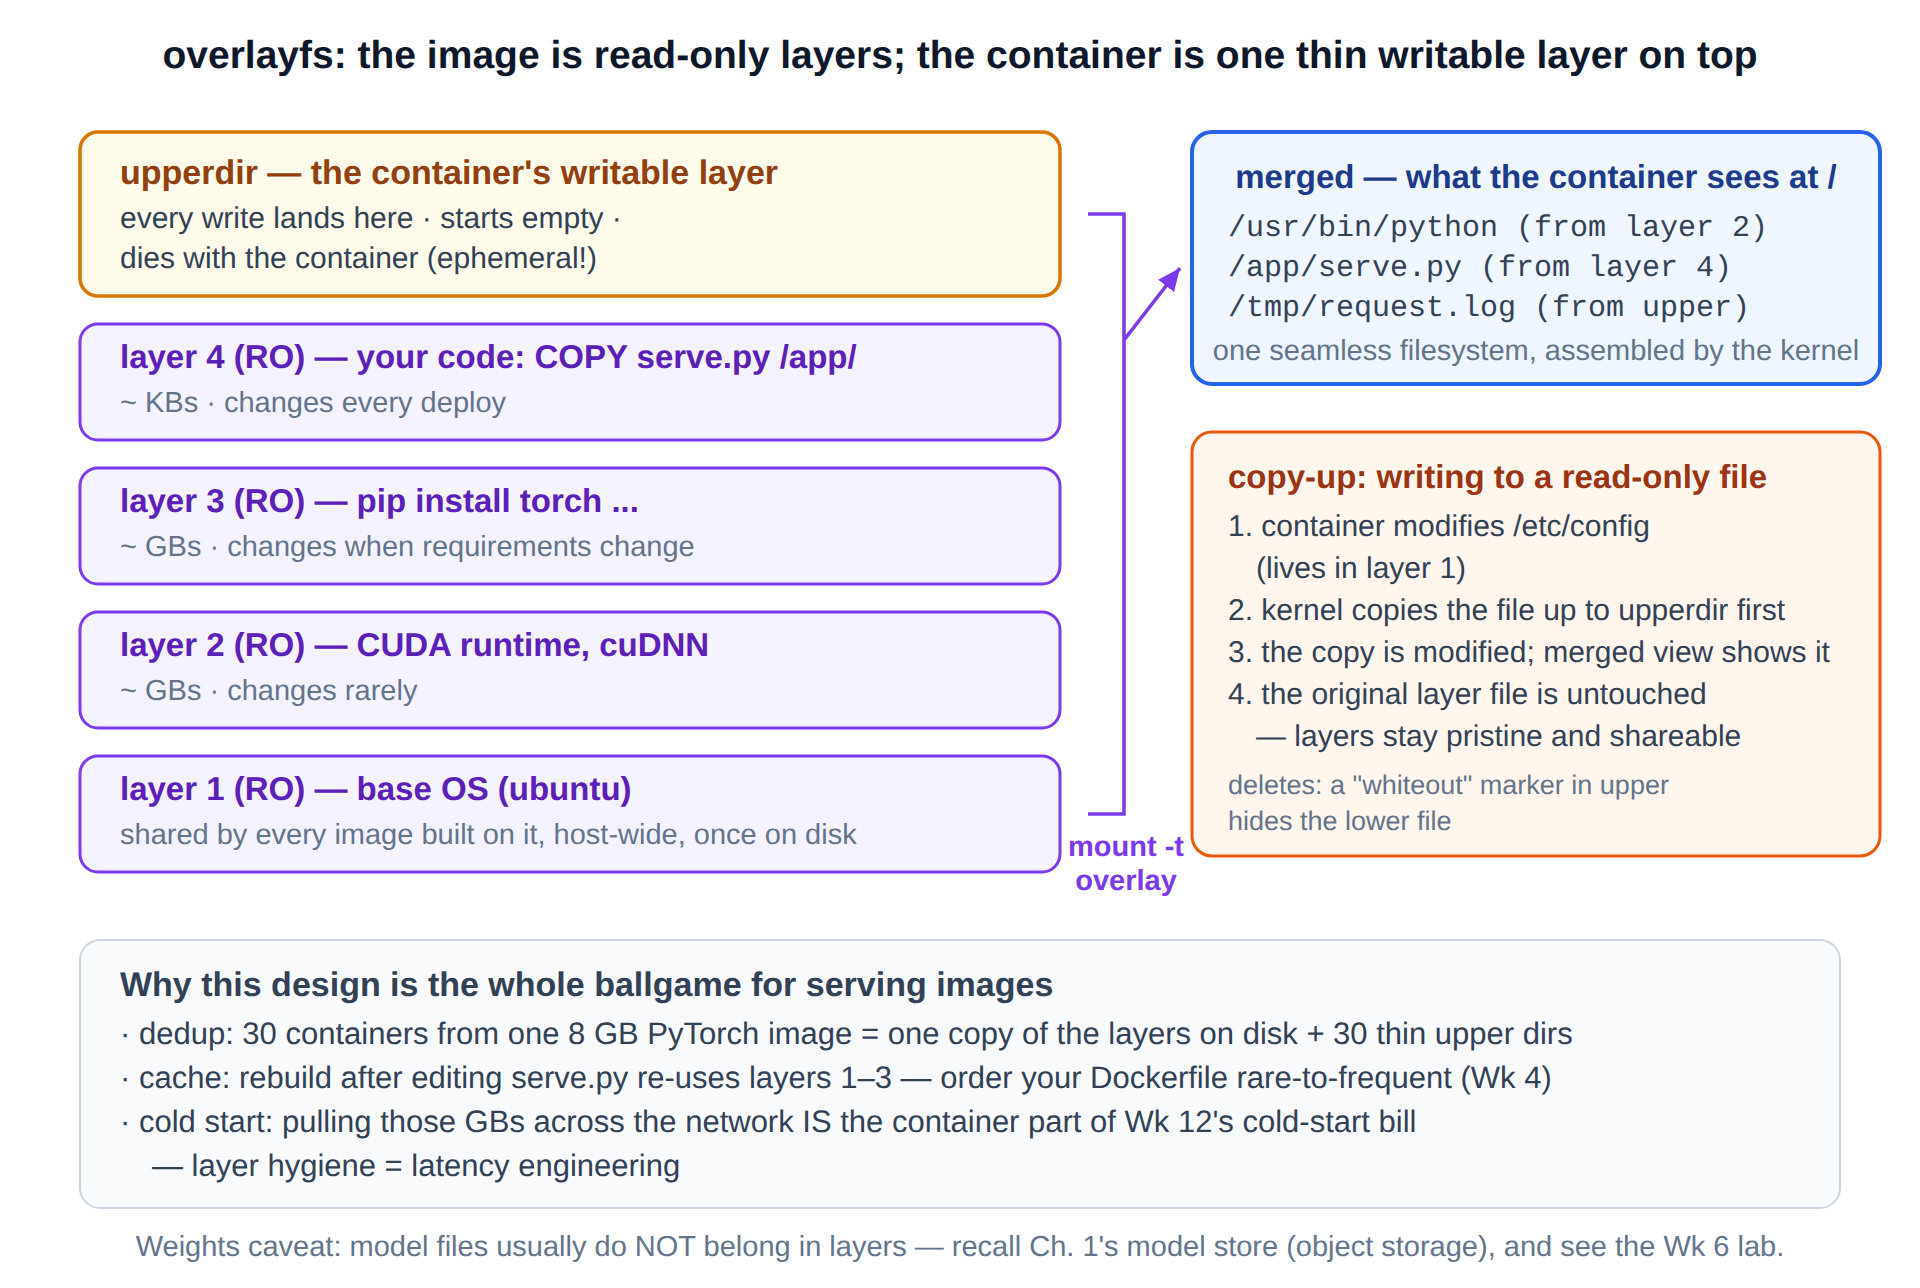
\includegraphics{figures/fig3-5_overlayfs.png}}\\[3pt]
  \figcaption{그림 3-5  overlayfs: 읽기 전용 이미지 계층 + 얇은 쓰기 가능 계층 하나 = 컨테이너의 루트. 쓰기는 copy-up하고 삭제는 whiteout을 남기며 계층은 깨끗한 공유 상태를 유지한다.}
\end{tbbfigure}

\subsection*{90초 만에 시연하는 세 가지 규칙}

overlayfs는 모든 기본 Linux 커널에 있는 마운트 유형이므로 Docker 없이 임시 디렉터리에서 전체 과정을 실험할 수 있다. 아래 기록은 실제로 실행해 볼 가치가 있다. 각 명령이 세 규칙 중 하나를 가르친다.

\begin{terminalbox}
\begin{Verbatim}[breaklines=true,breakanywhere=true,fontsize=\small,formatcom=\color{tbbtermfg},codes=\tbbcodeactive]
$ mkdir lower upper work merged
$ echo "from the image"  > lower/config.txt
$ echo "also the image"  > lower/keep.txt
$ sudo mount -t overlay overlay \
    -o lowerdir=lower,upperdir=upper,workdir=work merged
$ cat merged/config.txt                # RULE 1 - reads fall through
from the image
$ echo "changed!" > merged/config.txt  # RULE 2 - writes copy-up
$ cat lower/config.txt                 #   the layer is untouched...
from the image
$ ls upper/                            #   ...the copy lives in upper
config.txt
$ rm merged/keep.txt                   # RULE 3 - deletes leave whiteouts
$ ls -l upper/keep.txt
c--------- 1 root root 0, 0 ... upper/keep.txt   # a marker, not a file
$ ls lower/                            #   the bytes still exist below!
config.txt  keep.txt
\end{Verbatim}
\end{terminalbox}
\figcaption{기록 3-6  한 번에 보는 overlayfs. 읽기는 스택을 통과하고, 쓰기는 파일을 위로 복사한 뒤 수정하며, 삭제는 whiteout 표식으로 파일을 숨긴다. lower 계층은 깨끗하고 공유 가능한 상태를 유지한다.}

세 규칙의 결과를 분명히 해 보자. \textbf{읽기는 위에서 아래로 찾으므로} merged 관점에는 각 경로의 가장 위 버전이 보인다. 뒤 계층이 앞 계층을 수정하지 않고 파일을 "갱신"하는 방식이다. \textbf{쓰기는 copy-up을 일으킨다.} 먼저 파일 전체를 upper 디렉터리로 복사하고 그 사본을 바꾼다. 컨테이너마다 자체 upper가 있으므로 컨테이너 30개가 같은 기본 이미지의 모든 읽기 전용 바이트를 공유하면서도 그 이미지를 각각 "수정"할 수 있다. \textbf{삭제는 whiteout을 남긴다.} 문자 장치 표식(\code{c---------}, 장치 0:0)이 merged 관점에서 \code{keep.txt}를 숨기지만 바이트는 lower 계층에 남는다. whiteout 규칙에는 유명한 비용상 결과가 있다. \textbf{뒤 Dockerfile 계층의 RUN rm은 이미지를 줄이는 것이 아니라 늘린다.} "삭제한" 바이트가 앞 계층에 실려 가고 표식까지 더해진다. 파일을 만든 \textit{바로 그 계층에서} 삭제해야 하며, Dockerfile에서는 같은 \code{RUN} 줄을 뜻한다.

\begin{terminalbox}
\begin{Verbatim}[breaklines=true,breakanywhere=true,fontsize=\small,formatcom=\color{tbbtermfg},codes=\tbbcodeactive]
# WRONG - image contains 900MB of downloads AND a whiteout hiding them:
RUN apt-get install -y build-essential
RUN rm -rf /var/lib/apt/lists /tmp/downloads

# RIGHT - the layer never contains the junk at all:
RUN apt-get install -y build-essential && \
    rm -rf /var/lib/apt/lists /tmp/downloads
\end{Verbatim}
\end{terminalbox}
\figcaption{기록 3-7  Dockerfile 실무의 whiteout 규칙. 정리 작업은 치울 대상을 만든 RUN과 같아야 하며, 그렇지 않으면 바이트가 그대로 운반된다.}

\subsection*{계층이 경제적 설계인 이유 — 서빙 이미지를 장부로 읽기}

4주 차 실습에서 실제로 만들 이미지를 이용해 경제학자의 눈으로 스택을 읽어 보자. 서빙 이미지는 \textit{변경 속도}에 따라 자연스럽게 나뉘며, 순서를 잘 잡은 Dockerfile은 가장 천천히 바뀌는 내용을 가장 아래에 둔다.

\begin{tbbtablewrap}
  \begin{tabular}{@{}>{\raggedright\arraybackslash}m{\dimexpr 0.3617\tbltextwidth-2\tabcolsep\relax} >{\raggedright\arraybackslash}m{\dimexpr 0.1809\tbltextwidth-2\tabcolsep\relax} >{\raggedright\arraybackslash}m{\dimexpr 0.2234\tbltextwidth-2\tabcolsep\relax} >{\raggedright\arraybackslash}m{\dimexpr 0.2340\tbltextwidth-2\tabcolsep\relax}@{}}
  \arrayrulecolor{tbbnavy}\specialrule{1pt}{0pt}{0pt}
  \rowcolor{tbbtablehead}{\centering \bfseries\color{tbbnavy}계층(Dockerfile 단계)} & {\centering \bfseries\color{tbbnavy}일반적 크기} & {\centering \bfseries\color{tbbnavy}변경 주기} & {\centering \bfseries\color{tbbnavy}재빌드/가져오기 비용} \\
  \arrayrulecolor{tbbnavy}\specialrule{0.7pt}{0pt}{2pt}
  {FROM ubuntu / python-slim 기본 이미지} & {\textasciitilde{}80–150 MB} & {매년} & {거의 영구 캐시} \\
  \arrayrulecolor{tbbtableborder}\hline
  {CUDA 런타임 + cuDNN 라이브러리} & {\textasciitilde{}2–3 GB} & {CUDA 업그레이드마다} & {수개월 캐시} \\
  \arrayrulecolor{tbbtableborder}\hline
  {pip install torch + 종속성} & {\textasciitilde{}2–3 GB} & {requirements.txt 변경 시} & {수주 캐시} \\
  \arrayrulecolor{tbbtableborder}\hline
  {\textbf{COPY serve.py /app/}} & {\textbf{\textasciitilde{}40 KB}} & {\textbf{배포마다}} & {\textbf{수초}} \\
  \arrayrulecolor{tbbnavy}\specialrule{1pt}{2pt}{0pt}
  \end{tabular}\par
  \figcaption{표 3-3  계층별 모델 서버 이미지(대표 크기)}
\end{tbbtablewrap}

이 순서 덕분에 이 책 내내 두고두고 덕을 보는 세 가지가 생긴다. \textbf{중복 제거:} 노드 하나에 \textasciitilde{}5–6 GB 이미지의 레플리카 30개를 두어도 계층은 \textit{한 번만} 저장하고 거의 비어 있는 upper 디렉터리 30개만 더한다. ML 이미지로 컨테이너 밀도를 확보할 수 있는 이유다. \textbf{캐시:} \code{serve.py}를 편집하고 재빌드하면 아래의 모든 계층을 재사용한다. 재빌드는 수초, 푸시는 수 킬로바이트에 그친다. 반면 \code{COPY . /\allowbreak app}이 \code{pip install} \textit{위에} 있는 초보자의 고전적인 순서 역전에서는 모든 코드 편집이 종속성 계층을 무효화하고 torch를 다시 빌드하므로 20분과 수 기가바이트가 드는 재앙이 된다. \textbf{시작:} 컨테이너 파일 시스템의 "시작"은 이미 존재하는 계층을 overlay로 한 번 마운트하는 일이므로 밀리초밖에 걸리지 않는다. 파일 시스템 자체는 콜드 스타트 문제가 아니다. \textit{없는 계층을 네트워크로 가져오는 일이 문제다.} 12주 차를 미리 보는 계산을 해 보자. 새 노드에 6 GB 이미지를 유효 100–250 MB/s로 가져오면 레지스트리, 네트워크, 압축 해제가 모두 파이프에 부담을 주어 \textbf{코드 한 줄 실행 전에 콜드 스타트 25–60초}가 걸린다. 대개 단일 항목으로는 최대이며, 계층 위생이 정리 정돈이 아니라 지연 시간 엔지니어링인 이유다.

서빙에 특화된 한 가지 주의 사항으로 그림을 완성하자. \textbf{모델 가중치는 보통 이미지 계층에 넣지 않는다.} 가중치는 거대하고 코드와 다른 주기로 바뀌며, 제1장에서 배웠듯 객체 스토리지의 모델 저장소에 두고 시작할 때 로드하는 편이 맞다. 6주 차 실습에서 바로 그 경로를 만들며, 13주 차 레지스트리/버전 관리 이야기도 이에 의존한다. 30 GB 체크포인트를 계층에 구우면 모델 버전과 이미지 버전이 결합되고, 모든 노드의 디스크가 부풀며, 배포할 때마다 바뀌지 않은 수 기가바이트를 다시 보낸다. 불변 데모 이미지나 엣지 장비에서는 때때로 옳지만, 기본값이 아니라 의식적인 결정이어야 한다.

\begin{calloutbox}{tbbpurple}{tbbpurplefill}
{\normalsize\bfseries\color{tbbpurple}생각해 보기}\par\vspace{3pt}
\begin{tbbitemize}
  \item 팀원의 Dockerfile이 FROM python-slim → COPY . /app → pip install -r /app/requirements.txt → CMD ... 순서다. (a) serve.py 변경, (b) requirements.txt 변경 시 재빌드 동작을 예측하라. 올바르게 순서를 바꾸고 각 경우의 새 비용을 설명하라.
  \item 기록 3-6의 규칙을 이용해 보자. 같은 이미지의 컨테이너 두 개가 내부의 /var/log/app.log에 각각 내용을 덧붙인다. 서로의 줄이 보이는가? 두 파일은 물리적으로 어디에 존재하는가? 컨테이너를 제거하면 둘은 어떻게 되는가?
  \item 팀이 serve.py (40 KB)만 바뀌는 5.5 GB 이미지를 하루 6번 배포한다고 하자. 올바르게 계층화하면 배포마다 몇 바이트가 이동하는가? COPY가 pip 위에 있는 순서 역전에서는 어떠한가? (레지스트리 송신에도 요금이 부과되므로 제1장의 비용 관점을 적용한다.)
\end{tbbitemize}
\end{calloutbox}

\section{직접 만들기 — Docker가 실제로 더하는 것}

맨손으로 레시피를 조립할 시간이다. 아래 순서는 이번 주 실습의 지적 핵심이며 Liz Rice의 유명한 "Containers from Scratch" 시연 구조를 따른다. Rice는 Go로 라이브 코딩하지만, 우리는 신비를 더 벗겨 주는 기본 셸 명령으로 실행한다. 이 장의 각 절을 활용하는 다섯 단계다(그림 3-6). 순서대로 실행하고 모든 출력을 읽자.

\begin{tbbfigure}
  \adjustbox{max width=0.94\linewidth,max totalheight=0.46\textheight}{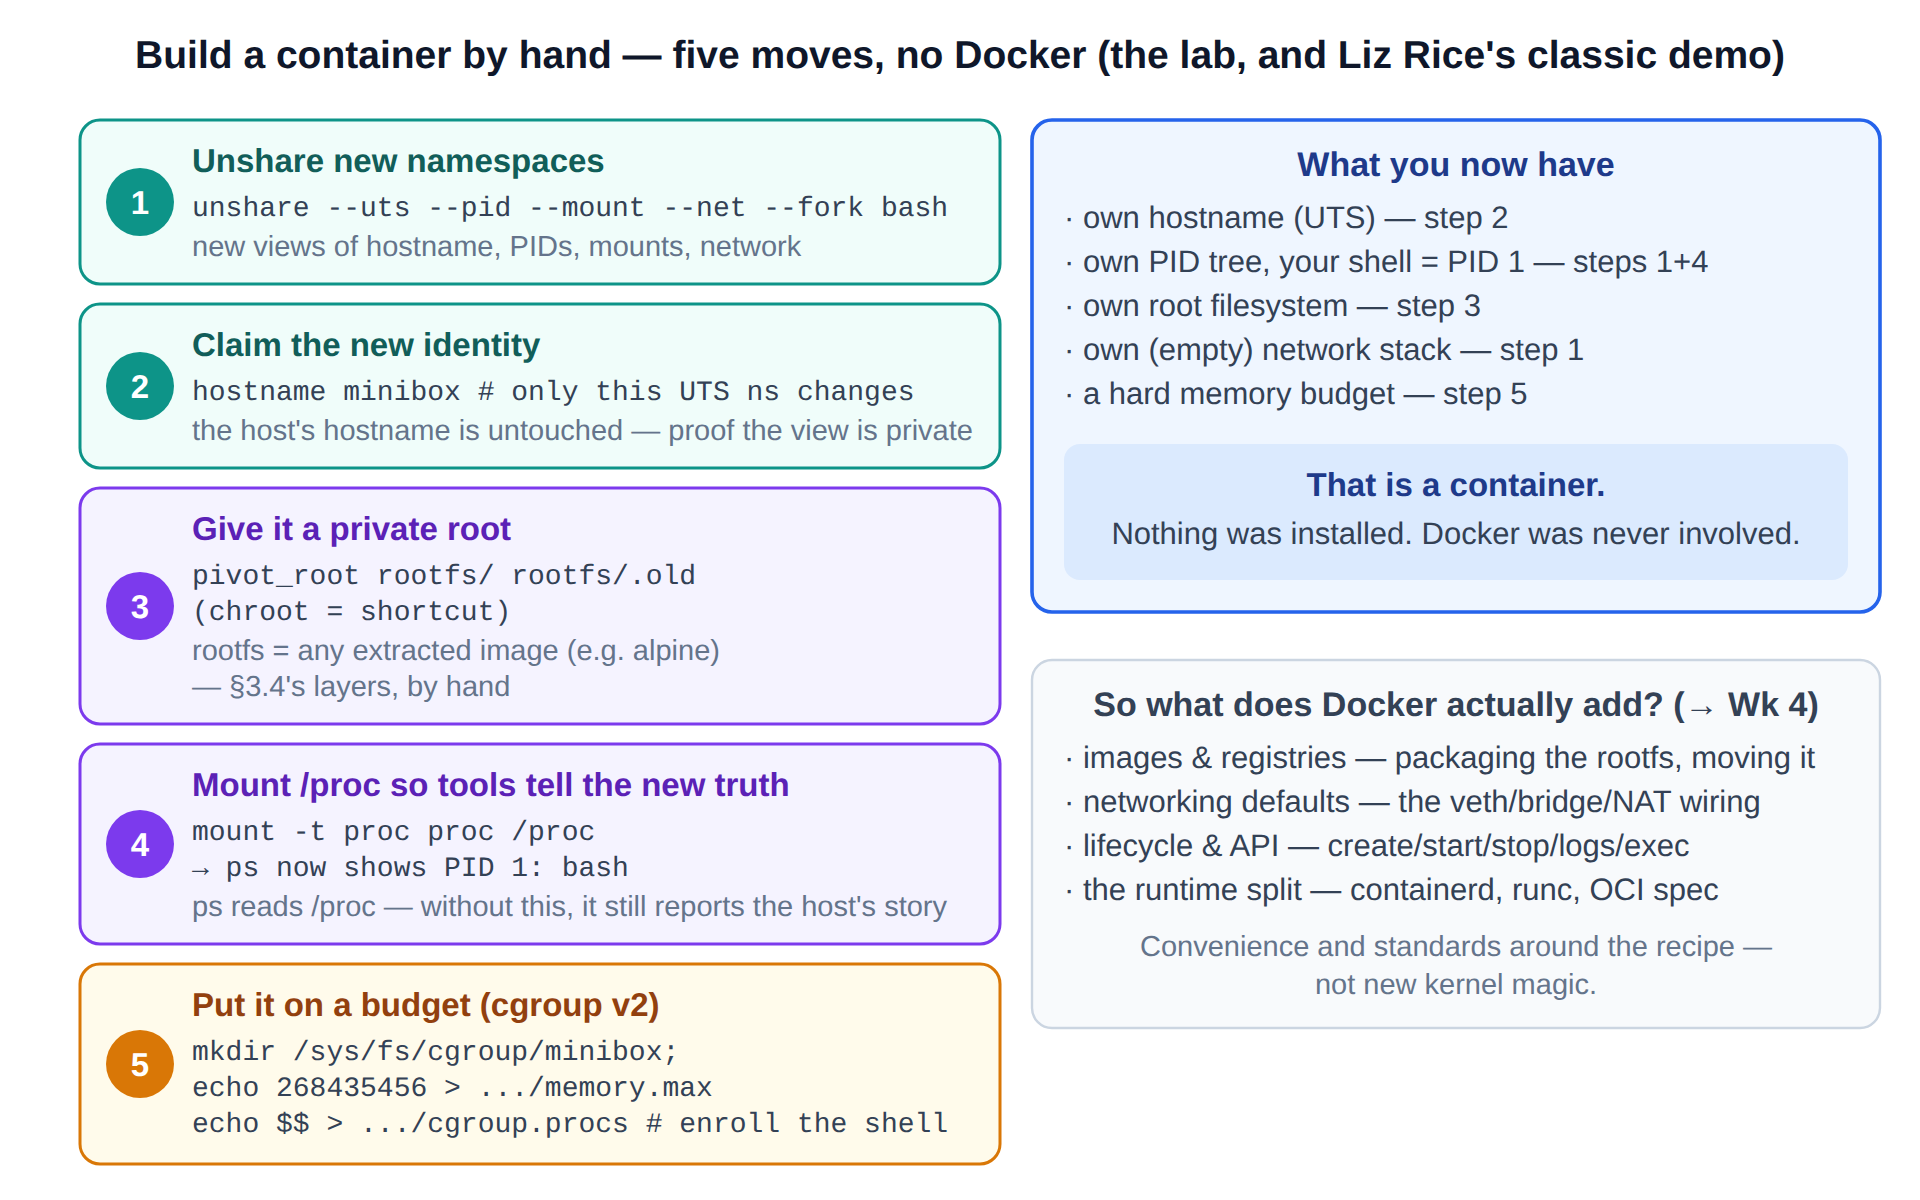
\includegraphics{figures/fig3-6_byhand.png}}\\[3pt]
  \figcaption{그림 3-6  다섯 단계로 만드는 컨테이너. 네임스페이스를 unshare하고, 신원을 얻고, 비공개 루트로 pivot하며, /proc를 마운트하고, cgroup에 등록한다. Docker가 더하는 것은 편의성과 표준이지 커널 마법이 아니다.}
\end{tbbfigure}

\subsection*{1\textasciitilde{}2단계: 새로운 관점과 비공개임을 보여 주는 증거}

\begin{terminalbox}
\begin{Verbatim}[breaklines=true,breakanywhere=true,fontsize=\small,formatcom=\color{tbbtermfg},codes=\tbbcodeactive]
$ sudo unshare --uts --pid --mount --net --fork bash   # MOVE 1
# (prompt looks identical - but check your namespace links vs Transcript 3-2)
$ hostname minibox                                     # MOVE 2
$ hostname
minibox
# ...meanwhile, in a second terminal on the host:
$ hostname
gpu-node-17                    # untouched. The view really is private.
\end{Verbatim}
\end{terminalbox}
\figcaption{기록 3-8  1\textasciitilde{}2단계. PID 소속은 자식에게 적용되므로 --fork가 중요하다. 터미널 두 개의 호스트 이름 대비가 첫 실습 아티팩트다.}

\subsection*{3단계: 비공개 루트(pivot\_root를 쓰고 chroot를 쓰지 않는 이유)}

alpine이나 ubuntu-base tar 아카이브 같은 소형 rootfs를 풀어 \code{/\allowbreak }로 만든다. rootfs는 문자 그대로 이미지 계층을 디렉터리 하나로 평탄화한 것이다. 시연에서는 \code{chroot}라는 지름길을 쓰며 실습에는 충분하다. 실제 런타임은 \code{pivot\_root}를 사용한다. 둘의 차이는 보안 소양을 위해 한 문장으로 정리할 가치가 있다. \code{chroot}는 프로세스가 생각하는 \code{/\allowbreak }의 위치만 \textit{다시 가리키고} 기존 루트는 마운트 네임스페이스에 남기므로 잘 알려진 탈출 묘수로 다시 접근할 수 있다. 감옥 밖 파일 디스크립터를 가진 프로세스는 되돌아 나갈 수 있다. 반면 \code{pivot\_root}는 마운트 네임스페이스의 루트를 \textit{교체}하며 기존 세계를 완전히 언마운트할 수 있다. 다시 가리키기냐 통째로 갈아 끼우기냐 — 고전적인 컨테이너 보안 상식 하나가 이제 당신 것이 되었다.

\begin{terminalbox}
\begin{Verbatim}[breaklines=true,breakanywhere=true,fontsize=\small,formatcom=\color{tbbtermfg},codes=\tbbcodeactive]
$ curl -LO https://.../alpine-minirootfs-3.20-x86_64.tar.gz   # ~3 MB(!)
$ mkdir rootfs && tar -xzf alpine-minirootfs-*.tar.gz -C rootfs
$ ls rootfs
bin  dev  etc  home  lib  ...  usr  var        # a whole tiny Linux userland
$ chroot rootfs /bin/sh                        # MOVE 3 (lab shortcut)
/ # ls /                                       # your / is now the rootfs
bin  dev  etc  home  lib  ...  usr  var
\end{Verbatim}
\end{terminalbox}
\figcaption{기록 3-9  3단계. rootfs는 그저 디렉터리이고 이미지는 계층으로 운반되는 rootfs다. Alpine은 3 MB이며 6 GB CUDA 이미지를 바라볼 기준을 제공한다.}

\subsection*{4단계: 도구가 새로운 진실을 말하게 하기}

\begin{terminalbox}
\begin{Verbatim}[breaklines=true,breakanywhere=true,fontsize=\small,formatcom=\color{tbbtermfg},codes=\tbbcodeactive]
/ # ps aux                       # BEFORE mounting /proc: confusion
ps: can't open /proc: No such file or directory
/ # mount -t proc proc /proc     # MOVE 4
/ # ps aux
PID   USER   COMMAND
  1   root   /bin/sh             # there it is: you are init
  9   root   ps aux
\end{Verbatim}
\end{terminalbox}
\figcaption{기록 3-10  4단계. ps는 /proc를 읽는다. 네임스페이스를 인식하는 proc를 마운트하면 도구가 프로세스 두 개와 PID 1인 셸이라는 새로운 세계를 보고한다.}

\subsection*{5단계: 예산과 전체 목록}

호스트의 두 번째 터미널에서 기록 3-4와 똑같이 cgroup을 만든다. \code{mkdir /\allowbreak sys/\allowbreak fs/\allowbreak cgroup/\allowbreak minibox}를 실행하고 \code{memory.max}에 \code{268435456}을 쓰며, 셸의 호스트 PID를 \code{cgroup.procs}에 쓴다. 이제 직접 만든 컨테이너에는 256 MiB 하드 벽이 생겼으며, 실습 B부에서 의도적으로 부딪힌다. 이 순간 존재하는 것을 목록으로 정리해 보자. 자체 호스트 이름(UTS), 자신이 init인 자체 PID 트리(PID), 자체 마운트 테이블과 루트 파일 시스템(MNT + rootfs), 아직 비어 있는 자체 네트워크 스택(NET), 단단한 메모리 예산(cgroup)을 가진 프로세스다. \textbf{이것이 컨테이너다.} 아무것도 설치하지 않았고 데몬도 실행되지 않았으며 Docker는 관여하지 않았다. 사용한 도구는 \code{unshare}, \code{chroot}, \code{mount}, \code{mkdir}, \code{echo}, 3 MB tar 아카이브가 전부다.

\subsection*{그렇다면 Docker가 실제로 더하는 것은 무엇인가?}

레시피 주위의 모든 것을 더하지만 커널 안에는 아무것도 더하지 않는다. \textbf{이미지와 레지스트리:} rootfs를 내용 주소화 계층으로 패키징하는 표준 방식이다. 각 계층은 바이트의 SHA-256으로 이름을 붙이므로 계층 캐시를 신뢰할 수 있다. 네트워크로 옮기고 어느 머신에서든 바이트까지 똑같이 재현하여 "내 노트북에서 작동한다"를 "GPU 노드에서도 작동한다"로 바꾼다. \textbf{네트워킹 기본값:} §3.2의 veth/브리지/NAT 배선을 컨테이너마다 만들고 제거하므로 \code{ip link add}를 직접 입력할 필요가 없다. \textbf{수명 주기와 API:} tmux 창에 unshare를 잔뜩 쌓는 대신 재시작 정책과 로그 캡처를 갖춘 데몬 기반 API로 create/start/stop/exec/logs를 제공한다. 그리고 \textbf{런타임 분리:} Docker 자체는 실제 레시피 실행을 아래로 위임한다. Docker → \code{containerd}(수명 주기 관리자) → \code{runc}로 이어진다. runc는 다섯 단계를 엄격하게 수행하는 것이 \textit{유일한 임무}인 작은 독립 실행 바이너리다. 어느 네임스페이스를 unshare할지, 어떤 cgroup 값을 쓸지, 어느 rootfs로 pivot할지를 지정하는 JSON 파일(OCI 런타임 명세)이 구동하며, 이 장을 설정 파일로 옮겨 적은 것처럼 읽힌다. 이 표준화된 바닥 계층 덕분에 제2장의 Kata와 gVisor가 Kubernetes 아래에서 대체재로 끼어들 수 있다. 바로 다음 주의 주제이며, 이 책이 아껴 둔 질문인 GPU를 상자 안에 주입하는 방식도 다룬다.

\begin{calloutbox}{tbbpurple}{tbbpurplefill}
{\normalsize\bfseries\color{tbbpurple}생각해 보기}\par\vspace{3pt}
\begin{tbbitemize}
  \item 직접 만든 컨테이너에서는 인터페이스를 올리기 전까지 localhost에도 ping이 실패한다. 호스트까지 작동하는 네트워킹을 제공하는 데 필요한 최소 추가 단계를 나열해 보자. (§3.2의 패킷 순회에 모든 부품이 있다. 쌍, 주소, up이 필요하다.)
  \item 직접 만든 컨테이너와 docker run alpine sh는 모두 같은 rootfs를 제공한다. Docker 버전에는 있지만 직접 만든 것에는 없는 운영상 중요한 요소 두 가지와 바이트 단위로 동일한 요소 하나를 제시하라.
  \item 해시(sha256)로 계층을 내용 주소화하면 서로 만난 적 없는 머신 사이에서도 계층 캐싱이 안전한 이유는 무엇인가? 부수적으로 어떤 공격을 막는가?
\end{tbbitemize}
\end{calloutbox}

\section{심판이 모델을 죽일 때: OOM 대응 지침}

이 장의 모든 메커니즘은 프로덕션의 한순간으로 모인다. 이 책에서 절 하나를 온전히 할애할 만큼 흔한 상황이다. 추론 서버가 실행되고 트래픽이 흐르다가 프로세스가 사라진다. 스택 추적도 마지막 로그 줄도 없으며 애플리케이션 텔레메트리에는 침묵만 남는다. 어딘가에서 재시작 루프가 시작된다. 이것이 컨테이너화된 모델 서버가 죽는 단연 가장 흔한 방식인 \textbf{OOM 강제 종료}다. 이 절을 마치면 진단하기 가장 쉬운 문제 중 하나가 된다(그림 3-7).

\begin{tbbfigure}
  \adjustbox{max width=0.94\linewidth,max totalheight=0.46\textheight}{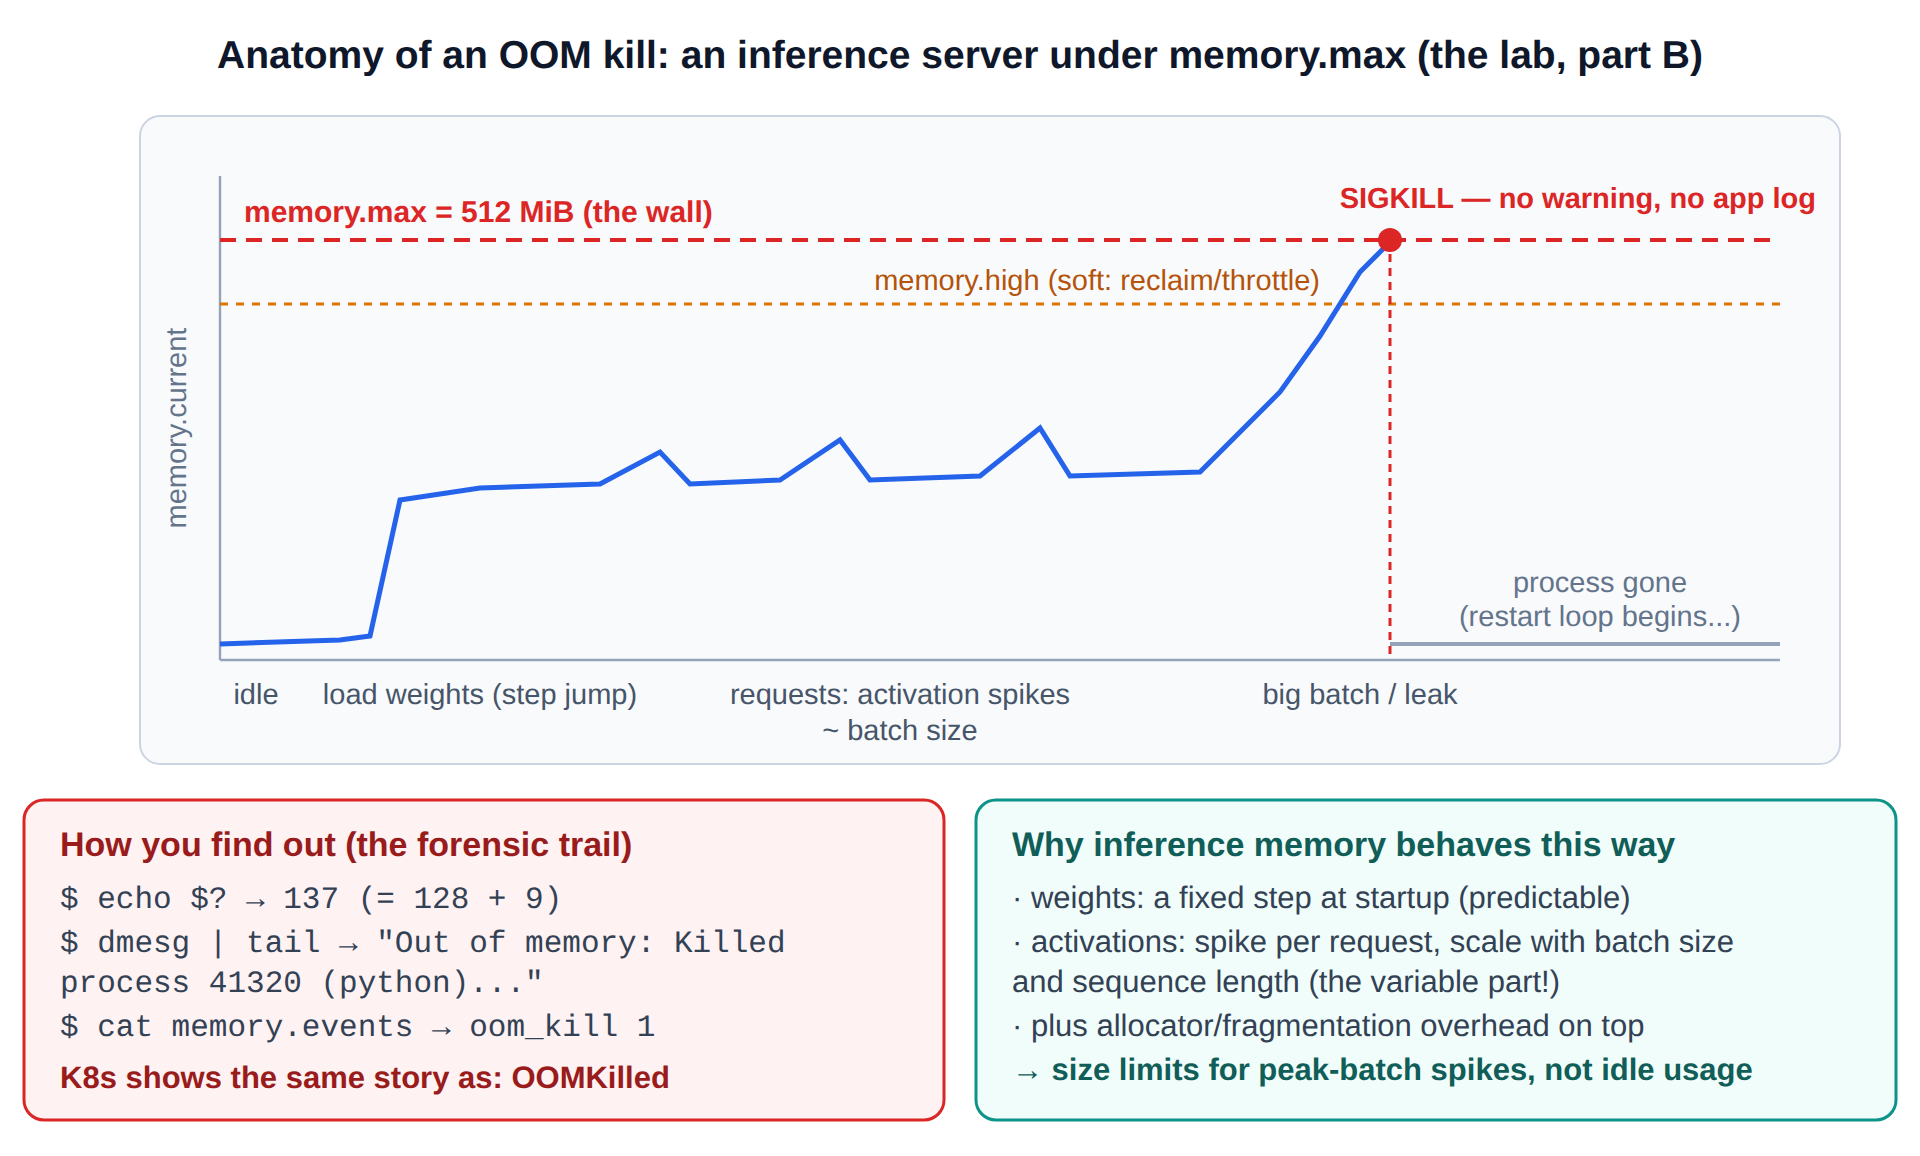
\includegraphics{figures/fig3-7_oom.png}}\\[3pt]
  \figcaption{그림 3-7  memory.max 아래에서 살아가는 추론 서버의 메모리 생애. 가중치 계단, 요청별 활성값 급증, 치명적인 경계 초과, 포렌식 흔적(137, dmesg, memory.events)을 보여 준다.}
\end{tbbfigure}

\subsection*{처음부터 끝까지 보는 메커니즘}

3.3절의 규칙을 시간순으로 되짚어 보자. 그룹의 \code{memory.current}가 \code{memory.max}를 향해 올라간다. 커널은 회수할 수 있는 것부터 회수하며 페이지 캐시가 먼저다. 그래서 파일 I/O가 많은 단계는 한도에 붙어도 해롭지 않을 수 있다. 메모리 회수 후에도 새 \textbf{익명} 할당(힙, 텐서)을 충족할 수 없으면 커널이 \textbf{cgroup 범위의 OOM 킬러}를 호출한다. 그룹의 프로세스에 본질적으로 메모리 사용량을 기준으로 점수를 매기고(\code{oom\_score\_adj}로 조정할 수 있다), 가장 큰 것을 고른다. 모델 서버 pod에서는 사실상 항상 모델 서버다. 그리고 \textbf{SIGKILL}을 보낸다. SIGKILL은 잡거나 막거나 처리할 수 없다. 정리도 플러시도 작별 인사도 없다. 따라서 증거는 피해자의 \textit{바깥에만} 남는다. 오전 2시에 필요해지기 전에 각 아티팩트를 눈으로 알아볼 수 있어야 한다.

\begin{terminalbox}
\begin{Verbatim}[breaklines=true,breakanywhere=true,fontsize=\small,formatcom=\color{tbbtermfg},codes=\tbbcodeactive]
$ echo $?                          # 1) the exit code, wherever the process ran
137                                #    = 128 + 9 (killed by signal 9, SIGKILL)
$ sudo dmesg | grep -i -A1 "out of memory"     # 2) the kernel's confession
Memory cgroup out of memory: Killed process 41320 (python)
  total-vm:1892456kB, anon-rss:498112kB, file-rss:1024kB, ...
$ cat /sys/fs/cgroup/.../memory.events          # 3) the cgroup's ledger
oom 3
oom_kill 1
# 4) and the same story, as Kubernetes tells it (Week 5):
$ kubectl describe pod model-server-7d4b9 | grep -A3 "Last State"
Last State:   Terminated
  Reason:     OOMKilled
  Exit Code:  137
\end{Verbatim}
\end{terminalbox}
\figcaption{기록 3-11  완전한 OOM 증거 사슬. 종료 코드 137, 한도에 가까운 회수 불가능 메모리 anon-rss가 보이는 dmesg 줄, oom\_kill 카운터, 그리고 세 가지를 되풀이하는 Kubernetes다.}

\code{dmesg} 줄에는 자세히 읽은 보람이 있는 세부 사항이 하나 있다. 512 MiB 한도에 \code{anon-rss:498112kB}다. 회수할 수 없는 \textit{익명} 메모리가 예산을 채워 kill이 일어났다. 캐시와 비슷한 \code{file-rss}는 메모리 회수가 이미 벗겨 냈기 때문에 작다. 커널이 자신의 자백에 인쇄한 3.3절의 메모리 회수 미묘함이다.

\subsection*{특히 추론 서버가 벽으로 걸어 들어가는 이유}

OOM 킬러가 형을 집행하지만 범죄는 거의 언제나 잘못 산정한 예산이다. 추론 메모리에는 무상태 웹 앱만 다루며 길러진 직관이 잘못 짚는 \textit{형태}가 있기 때문이다. 웹 핸들러는 평평한 기준선 주위에서 요청당 수 킬로바이트를 할당하므로 관측한 사용량 ≈ 필요한 사용량이고 "유휴 + 10\%"도 괜찮은 한도다. 추론 서버는 세 곡선이 겹친다. 시작할 때의 크고 고정된 \textbf{가중치} 계단(예측 가능하며 한 번 측정), 적당하고 일정한 평탄 구간, 그리고 트래픽에 의존해 \textbf{배치 크기와 시퀀스 길이에 비례하여 높아지는 요청별 활성값 급증}이다. 그 위에 할당자 오버헤드도 더해진다. PyTorch 캐싱 할당자는 해제된 블록을 풀에 보관하고 단편화가 더 늘린다. 평탄 구간만으로는 최대치에 관해 거의 아무것도 알 수 없다.

\begin{calloutbox}{tbbblue}{tbbbluefill}
{\normalsize\bfseries\color{tbbblue}계산 예시 — 소형 BERT 서버의 memory.max 산정(실습 규모 수치)}\par\vspace{3pt}
CPU에서 서빙하는 BERT-base 분류기를 생각해 보자. 실습 B부 워크로드와 비슷하다. 가중치는 110 M parameters × 4 bytes (fp32) ≈ \textbf{440 MB}이며 시작할 때 한 번 로드한다. 그림 3-7의 계단이다. 부하 상태에서 측정하면 다음과 같은 대표 수치가 나온다.

\begin{tbbitemize}
  \item 로드 후 유휴 상태: \textbf{\textasciitilde{}620 MB}(가중치 + 런타임 + 할당자 풀)
  \item batch 8 × seq 128: \textbf{\textasciitilde{}900 MB}까지 급증  ·  batch 32 × seq 256: \textbf{\textasciitilde{}1.4 GB}까지 급증
\end{tbbitemize}

정책을 비교해 보자. \textbf{단순 정책:} limit = 유휴 + 10\% ≈ \textbf{680 MiB} → \textit{첫} batch-8 요청에서 죽고 재시작 루프에 들어간다. 재시작할 때마다 440 MB 로드 비용을 다시 낸다. \textbf{최대치 기준:} limit = 측정한 최악 급증 × 1.25(여유) ≈ \textbf{1.75 GiB} → 부하 테스트한 모든 상황에서 살아남지만 레플리카당 유휴 상태보다 \textasciitilde{}1.1 GB를 더 예약한다. 제1장의 밀도와 비용 절충이다. \textbf{경계 설정:} 서버 구성에서 batch ≤ 8, seq ≤ 128로 서빙을 제한하고 limit ≈ 900 MB × 1.25 ≈ \textbf{1.1 GiB}로 둔다. 예약량은 줄고 최악 조건에는 경계가 생기지만 처리량 상한을 대가로 치른다. 지연 시간·처리량·비용 삼각형이 다시 등장한다. 단순하지 않은 두 정책은 모두 방어할 수 있지만, 단순 정책은 트래픽이라는 도화선을 단 시한폭탄이다.
\end{calloutbox}

\vspace{3.0pt}

정직성을 위해 두 가지를 분명히 하자. 첫째, 위 산술은 \textit{방법}이며 실제 수치는 달라진다. 대응 지침의 첫 동사가 추측이 아니라 \textbf{측정}인 이유다. 둘째, GPU 서빙에서는 같은 이야기가 두 번 반복된다. 커널 OOM은 이 절에서 설명한 그대로 호스트 RAM을 관리하지만, \textbf{GPU VRAM에는 다른 심판}이 있다. VRAM이 고갈되면 CUDA 할당자의 \code{torch.cuda.OutOfMemoryError}가 발생한다. SIGKILL이 아니라 할당자 오류이므로 Python에서 \textit{잡을 수 있고}, 해당 요청만 떨궈 낼 수 있다. 종료 코드 137 + dmesg와 Python 트레이스백이라는 징후로 두 OOM을 구분하는 것은 실제로 유용한 진단 기술이다. 11주 차에는 VRAM 쪽에서 계속 커지는 세 번째 등장인물인 KV 캐시를 더한다.

\subsection*{대응 지침}

\begin{tbbitemize}
  \item \textbf{평탄 구간이 아니라 최대치에 맞춰 산정한다.} 구성 가능한 최대 배치와 가장 긴 시퀀스를 사용하는 \textit{최악 조건 부하 테스트}에서 \code{memory.current}를 측정한다. 9주 차 Locust 실행이 정확히 이를 만든다. 명시적인 여유 용량을 더해 그 최대치보다 높게 \code{memory.max}를 설정한다(예시는 1.25× 사용). 유휴 관찰로 한도를 도출해서는 안 된다.
  \item \textbf{가변 부분에 경계를 둔다.} 급증은 배치와 시퀀스 길이에 비례한다. 서버 구성에서 둘을 제한하면 상한 없던 메모리 동작에 상한이 생기고, 앞 단계의 "최악 조건"이 실제로 존재하는 숫자가 된다. 제1장의 SLO 사고를 메모리에 적용한 것이다.
  \item \textbf{memory.high를 경보선으로 사용한다.} max보다 아래에 설정하고(예: 1.75 GiB max 아래 high = 1.5 GiB) \code{memory.events} / 메모리 압력 신호에 경보를 건다. 조용한 처형 대신 회수, 스로틀링, 증가하는 카운터가 있는 경고 단계를 그래프로 얻는다. 14주 차에 대시보드로 연결한다.
  \item \textbf{137을 수수께끼가 아니라 진단으로 읽는다.} 종료 코드 137 + memory.events의 \code{oom\_kill} = 버그가 아니라 예산 문제다. 해결을 논의할 때 나와야 할 말은 "크기를 조정하거나 경계를 둔다"이지 "try/except를 추가한다"가 아니다. SIGKILL은 잡을 수 없고, 계산 예시처럼 치명적인 할당이 자기 코드의 것이 아닐 때도 많다.
  \item \textbf{5주 차보다 먼저 Kubernetes에서 무엇이 무엇에 대응하는지 알아둔다.} requests는 스케줄러의 계획 수치이고 limits는 이 장의 cgroup 벽이다. QoS 클래스는 OOM \textit{우선순위} 정책이다. Guaranteed pod(requests = limits)는 가장 보호적인 \code{oom\_score\_adj}를 받고, \textit{노드}의 메모리가 부족하면 BestEffort pod가 가장 먼저 희생된다. 서빙 클러스터에서는 보통 swap을 끈다. 벽은 그대로 벽이다.
\end{tbbitemize}

\begin{calloutbox}{tbbpurple}{tbbpurplefill}
{\normalsize\bfseries\color{tbbpurple}생각해 보기}\par\vspace{3pt}
\begin{tbbitemize}
  \item 동료가 우아하게 성능을 낮추기 위해 Python에서 OOM을 잡자고 제안한다(try/except MemoryError). 메커니즘과 두 OOM의 차이를 이용해 (a) cgroup 벽에서는 작동할 수 없는 이유, (b) GPU 쪽에서 매우 비슷한 아이디어가 작동하는 곳을 설명하라.
  \item 서버에서 측정한 급증은 batch 32에서 1.9 GB, batch 64에서 3.4 GB다. 노드 용량상 레플리카당 한도는 2.5 GiB다. 계산 예시의 방법으로 구성을 제안하고, 지연 시간·처리량·비용 삼각형의 어느 꼭짓점을 희생했는지 밝혀라.
  \item 기록 3-11에서 dmesg가 대신 file-rss:400000kB와 anon-rss:90000kB를 보여 주었다고 하자. "OOM"에 관해 무엇을 알려 주며 해결책이 완전히 달라야 하는 이유는 무엇인가?
\end{tbbitemize}
\end{calloutbox}

\section{실습: 미니 컨테이너와 관찰한 OOM}

이번 주 실습은 상자를 만들고 그 벽에 부딪히는 이 장의 흐름을 반영한 두 부분으로 이루어진다. 어느 Linux VM이나 이 책의 클라우드 인스턴스에서도 실행할 수 있으며 GPU는 필요 없다. OOM 시연은 의도적으로 CPU만 사용하므로 비싼 인스턴스를 걸 필요가 없다. 안내서에는 정확한 명령이 있고, 이 절에서는 의도·프로토콜·예상 관찰 결과를 정해 실습에서 맹목적으로 입력하지 않고 예측을 \textit{확인}하게 한다. 산출물은 명령 기록의 핵심과 이 장의 절에 각각 연결한 관찰 세 가지를 담은 1쪽 보고서다.

\subsection*{A부 — 다섯 단계 실행하기}

기록 3-8부터 3-10까지 처음부터 끝까지 실행하며 아티팩트 네 가지를 수집한다. 첫째, 터미널 두 개의 \textbf{호스트 이름 대비}로 §3.2의 비공개 관점을 입증한다. 둘째, \code{/\allowbreak proc} 마운트 뒤 \textbf{PID 1 = 자기 셸이라고 표시하는 ps}로 §3.2의 두 가지 진실을 확인한다(마운트 \textit{전}의 \code{ps} 출력도 기록하자 — 그 오류 메시지가 바로 실전에서 만나는 "도구는 /proc를 읽는다"는 교훈이다). 셋째, 내부와 호스트 셸의 \code{ls -l /\allowbreak proc/\allowbreak \$\$/\allowbreak ns}를 비교해 모든 숫자가 다른지 확인하는 \textbf{네임스페이스 inode 비교}다(기록 3-2의 테스트를 직접 만든 컨테이너에 적용한다). 넷째, \code{cat /\allowbreak sys/\allowbreak fs/\allowbreak cgroup/\allowbreak minibox/\allowbreak cgroup.procs}가 컨테이너가 1이라고 믿는 프로세스의 \textit{호스트} PID를 출력하는 \textbf{호스트 쪽 예산 관점}이다. 마지막 아티팩트는 출력 한 줄에 이 장의 명제를 담는다. 같은 프로세스, 두 가지 진실, 하나의 예산이다.

\subsection*{B부 — 처형 관찰하기}

이제 서빙의 교훈을 살펴본다. 예산을 설정한 컨테이너 또는 \code{memory.max} = 256 MiB인 새 cgroup 안에서 안내서의 장난감 추론 스크립트를 실행한다. 의도적으로 큰 모델 객체를 로드한 뒤(가중치 계단) 점점 커지는 배치를 서빙한다(활성값 급증). 두 번째 터미널의 호스트에서 관찰한다.

\begin{terminalbox}
\begin{Verbatim}[breaklines=true,breakanywhere=true,fontsize=\small,formatcom=\color{tbbtermfg},codes=\tbbcodeactive]
# terminal 2 (host): watch the two files that matter, side by side
$ watch -n 0.5 'cat /sys/fs/cgroup/minibox/memory.current \
                 /sys/fs/cgroup/minibox/memory.events'
# you will watch Figure 3-7 draw itself:
#   ~8 MB (idle shell) -> ~120 MB (model loaded) -> spikes with each batch
#   -> at the fatal batch: memory.current snaps DOWN, oom_kill: 0 -> 1
# terminal 1 (container): the victim's-eye view
$ python toy_serve.py
loaded model (112.4 MB)
batch  4 ok   peak ~158 MB
batch 16 ok   peak ~214 MB
Killed                          # <- the shell says this, not Python
$ echo $?
137
\end{Verbatim}
\end{terminalbox}
\figcaption{기록 3-12  예상대로 펼쳐지는 B부. 신호를 보고하는 셸이 "Killed"라고 말하며 Python에는 마지막 말할 기회가 없다는 점에 주목한다. 이후 기록 3-11처럼 dmesg와 memory.events를 수집한다.}

관찰을 엔지니어링으로 바꾸는 후속 실험 두 가지를 실행한다. \textbf{(1)} \code{memory.high}를 200 MiB로 설정하고 반복한다. 강제 종료가 일어나기 전에 벽 앞 단계의 성격이 바뀐다. 진행이 느려지고 회수가 요동치며 \code{memory.events}의 메모리 압력 카운터가 증가한다. 경보선을 직접 경험하고 14주 차의 좋은 경보가 무엇에 반응하는지 미리 본다. \textbf{(2)} 스크립트 배치 크기를 살아남은 가장 큰 값으로 제한하고 같은 256 MiB 한도에서 전체 실행이 살아남는지 보인다. "가변 부분에 경계를 둔다"는 해결책을 직접 입증하며 계산 예시의 방법을 자체 수치로 뒷받침한다.

\begin{calloutbox}{tbbpurple}{tbbpurplefill}
{\normalsize\bfseries\color{tbbpurple}실습 체크리스트}\par\vspace{3pt}
\begin{tbbitemize}
  \item A부 아티팩트: 호스트 이름 대비 · /proc 마운트 전후 ps · 내부와 외부의 /proc/\$\$/ns · 호스트 쪽 cgroup.procs.
  \item B부 아티팩트: memory.current 시간 흐름(수기로 적어도 됨) · 종료 코드 137 · dmesg 줄(anon-rss 수치 인용) · memory.events 카운터.
  \item 후속 실험: memory.high 경고 단계의 동작 · 같은 한도에서 살아남는 배치 상한 재실행.
  \item 보고서: 각각 해당 절을 밝힌 관찰 세 가지(예: "proc 마운트 전에 ps 실패 — §3.2의 도구는 /proc를 읽는다는 교훈").
  \item 정리: 셸 종료, cgroup rmdir, rootfs 삭제. (이번 주에는 과금될 클라우드 자원이 없지만 제2장의 습관을 유지한다.)
\end{tbbitemize}
\end{calloutbox}

\vspace{3.0pt}

\begin{calloutbox}{tbbpurple}{tbbpurplefill}
{\normalsize\bfseries\color{tbbpurple}생각해 보기}\par\vspace{3pt}
\begin{tbbitemize}
  \item B부에서 강제 종료 전에 memory.current가 저절로 떨어질 때가 있다. 커널은 무엇을 하고 있으며 §3.3의 어떤 미묘함을 보여 주는가? 여기서 OOM을 늦추지만 막지는 못하는 이유는 무엇인가?
  \item 실행 전에 예측해 보자. 장난감 서버가 워커 두 개를 포크하고 치명적인 급증이 워커에서 발생하면 OOM 킬러는 어느 프로세스를 선택하며 이후 서버는 어떤 모습인가? (oom\_score가 힌트다. 실습에서 검증하고 tini의 회수 의무가 중요한 이유와 연결하라.)
\end{tbbitemize}
\end{calloutbox}

\namedsection{요약}{열 가지로 정리한 제3장}

\qitem{1}{\textbf{커널에는 컨테이너 객체가 없다.} 컨테이너는 공유 커널의 일반 프로세스를 네임스페이스(프로세스에 보이는 것) + cgroup(사용할 수 있는 것) + 계층형 파일 시스템(세계가 오는 곳)으로 감싸는 관례다. 제2장 격리 스펙트럼의 주의 사항을 이제 메커니즘으로 이해한다.}

\qitem{2}{\textbf{네임스페이스는 머신이 아니라 관점을 비공개로 만든다.} PID, NET, MNT, UTS, IPC, USER와 cgroup, 시간 네임스페이스가 있다. API는 unshare/clone/setns이며, \code{docker exec}는 겉모습만 바꾼 setns일 뿐이다.}

\qitem{3}{\textbf{PID 1은 직무다.} 고아를 회수하고 신호를 처리해야 한다. 그렇지 않으면 롤아웃(rollout)에서 SIGTERM이 무시되고 끝내 SIGKILL을 받는다. 서버에서 SIGTERM을 처리하거나 tini를 실행해야 한다. 이 한 문단이 실제 사고를 막는다.}

\qitem{4}{\textbf{NET 네임스페이스는 모든 컨테이너에 자체 포트 공간을 제공}하고, veth 쌍과 NAT를 통해 호스트 브리지에 연결한다. Kubernetes pod는 NET 네임스페이스 하나를 공유하는 컨테이너다. 그래서 localhost 사이드카와 pod당 IP 하나가 가능하다(5주 차).}

\qitem{5}{\textbf{cgroups v2는 예산의 파일 시스템이다.} 파일에 한도를 echo하고 PID를 등록한 뒤 사용량을 읽는다. Docker 플래그와 K8s 한도가 이 파일을 대필한다.}

\qitem{6}{\textbf{cpu.max는 뭉텅이로 스로틀링한다.} 프로세스가 창의 할당량을 소진하면 통째로 멈춘다. 프로파일러에는 보이지 않고 cpu.stat의 nr\_throttled에는 보이며 p99에 치명적이다. 제2장 스틸 타임의 사촌이다.}

\qitem{7}{\textbf{memory.max는 집행자가 지키는 벽이다.} 회수 실패 후 벽을 넘으면 OOM 킬러가 cgroup에서 가장 큰 프로세스에 SIGKILL을 보낸다. 종료 코드 137, dmesg 자백, memory.events oom\_kill, K8s "OOMKilled"가 남는다. 오류 경로가 아니라 직접 선택한 예산의 집행이다.}

\qitem{8}{\textbf{추론 메모리는 계단 + 평탄 구간 + 트래픽에 비례하는 급증}이다. 가중치 뒤에 배치/시퀀스에 의존하는 활성값이 온다. 측정한 최대치로 한도를 산정하고, 배치/길이에 경계를 두며, memory.high를 경보선으로 쓴다. 유휴 상태로 산정해서는 안 된다.}

\qitem{9}{\textbf{overlayfs는 이미지에 경제성을 제공한다.} 호스트 전체가 공유하는 읽기 전용 계층, 컨테이너당 하나의 얇은 쓰기 가능 upper, 쓰기 시 copy-up, 삭제 시 whiteout이다. 변경 속도에 따른 계층화 ⇒ 중복 제거, 빌드 캐시, 즉각적인 파일 시스템 시작이며, 이미지 가져오기가 실제 콜드 스타트 비용이다(12주 차). 가중치는 계층이 아니라 모델 저장소에 둔다.}

\qitem{10}{\textbf{다섯 단계로 컨테이너를 직접 만들 수 있다.} unshare, hostname, pivot\_root, /proc 마운트, cgroup이다. 따라서 Docker가 더하는 이미지/레지스트리, 네트워크 기본값, 수명 주기 API, 표준화된 런타임 분리(containerd/runc/OCI)가 무엇인지 정확히 안다. GPU 접근과 함께 4주 차의 주제다.}

\namedsection{연습문제}{}

\subsection*{A. 객관식}

\qitem{1}{컨테이너와 Linux 커널에 관한 설명으로 옳은 것은?}

\begin{tbboptions}
  \item ① 커널은 전용 시스템 호출로 만드는 컨테이너 객체를 제공한다
  \item ② 컨테이너는 커널이 스케줄링하는 일반 프로세스를 네임스페이스, cgroup, 마운트한 계층형 파일 시스템으로 감싼 것이다
  \item ③ 컨테이너는 경량 VM처럼 두 번째 커널을 실행한다
  \item ④ 컨테이너는 Docker 독점 커널 기능이다
\end{tbboptions}

\qitem{2}{컨테이너화 서버가 롤아웃 중 SIGTERM을 무시하고 유예 기간 뒤 SIGKILL을 받는다. 가장 가능성 높은 원인은?}

\begin{tbboptions}
  \item ① NET 네임스페이스가 외부 신호를 버린다
  \item ② CPU 스로틀링 시 cgroup이 신호 전달을 막는다
  \item ③ 서버가 PID 네임스페이스의 PID 1로 실행되면서 SIGTERM 핸들러를 설치하지 않았다. PID 1에는 기본 처리가 적용되지 않는다
  \item ④ overlayfs가 프로세스를 읽기 전용으로 만들었다
\end{tbboptions}

\qitem{3}{추론 컨테이너의 cpu.max를 "25000 100000"으로 설정했다. 부하 상태에서 가장 일치하는 관찰 결과는?}

\begin{tbboptions}
  \item ① 모든 요청이 균일하게 4× 느려진다
  \item ② p50은 거의 움직이지 않지만 cpu.stat의 nr\_throttled가 증가하면서 p99가 최대 \textasciitilde{}75 ms씩 급증한다
  \item ③ 컨테이너가 종료 코드 137로 죽는다
  \item ④ 아무 영향이 없다. cpu.max는 배치 작업에만 영향을 준다
\end{tbboptions}

\qitem{4}{pod가 애플리케이션 로그 없이 종료 코드 137로 죽고 memory.events에는 oom\_kill: 1이 나타난다. 가장 먼저 해야 할 올바른 해석은?}

\begin{tbboptions}
  \item ① 모델 런타임의 세그멘테이션 폴트이므로 상위 프로젝트에 버그를 보고한다
  \item ② 커널이 memory.max를 강제했다. 회수에 실패하자 OOM 킬러가 cgroup에서 가장 큰 프로세스에 SIGKILL을 보냈다
  \item ③ 가져오는 동안 이미지가 손상되었다
  \item ④ 디스크 부족으로 Kubernetes가 pod를 퇴거시켰다
\end{tbboptions}

\qitem{5}{노드 하나의 컨테이너 30개가 모두 같은 8 GB PyTorch 기본 이미지를 쓴다. 30번째 컨테이너의 파일 시스템에 추가되는 대략적인 디스크 용량은?}

\begin{tbboptions}
  \item ① \textasciitilde{}8 GB — 컨테이너마다 이미지를 복사한다
  \item ② \textasciitilde{}4 GB — 쓰기 시 복사(copy-on-write)가 절반으로 줄인다
  \item ③ \textasciitilde{}0 — 계층은 읽기 전용으로 공유하며 컨테이너마다 얇은 쓰기 가능 upper 디렉터리만 추가한다
  \item ④ memory.max에 따라 다르다
\end{tbboptions}

\qitem{6}{실제 컨테이너 런타임이 비공개 루트에 chroot 대신 pivot\_root를 사용하는 이유는?}

\begin{tbboptions}
  \item ① pivot\_root의 파일 I/O가 더 빠르다
  \item ② 네임스페이스 안에서는 chroot를 사용할 수 없다
  \item ③ pivot\_root는 실제로 마운트 네임스페이스의 루트를 교체하고 기존 루트를 분리한다. chroot는 경로만 다시 가리키며 설계상 탈출할 수 있다
  \item ④ pivot\_root가 rootfs를 압축한다
\end{tbboptions}

\subsection*{B. 단답형}

\qitem{1}{컨테이너 레시피의 세 재료와 각각의 역할을 한 구절로 쓰라.}

\qitem{2}{종료 코드 137을 산술적으로 해석하고 OOM 강제 종료가 프로세스 밖에서 증거를 남기는 두 위치를 쓰라.}

\qitem{3}{Kubernetes pod의 컨테이너 두 개가 localhost로 통신한다. 이를 위해 반드시 공유해야 하는 네임스페이스와 그 결과로 생기는 pod 속성은 무엇인가?}

\qitem{4}{Dockerfile의 \code{RUN rm -rf /\allowbreak opt/\allowbreak samples} 단계가 별도 계층에 있고 이미지 크기를 줄이지 못했다. 원인이 되는 overlayfs 메커니즘을 한 문장으로 설명하라.}

\subsection*{C. 서술형}

\qitem{1}{컨테이너를 직접 만드는 다섯 단계(§3.5)를 설명하라. 각 단계에서 이 장의 어느 메커니즘을 사용하며 작동을 입증하기 위해 어떤 관찰 가능한 증거를 수집할지 밝혀라. 직접 만든 컨테이너에는 없지만 Docker가 더하는 것 두 가지로 마무리하라.}

\qitem{2}{한도 2 GiB인 추론 pod가 트래픽 최대치 부근에서 거의 매일 OOM 강제 종료를 겪는다. 유휴 사용량은 1.1 GiB다. §3.6의 대응 지침으로 진단과 해결 계획을 작성하라. 무엇을 측정하고, 어떻게 크기를 조정하거나 경계를 두며, 어느 경보선을 설정할지, 각 단계가 제1장의 용어로 어떤 절충을 하는지 설명하라.}

\qitem{3}{"컨테이너가 승리한 것은 네임스페이스가 아니라 overlayfs 덕분이다." §3.4의 경제성(중복 제거, 캐시, 시작, 배포)과 §3.2–3.3의 격리 및 운영 속성을 이용해 이 주장에 찬성과 반대 논거를 제시하라. 최종 입장을 정하고 서빙 시스템과 관련된 관점에서 논증하라.}

\namedsection{정답 및 해설}{}

\subsection*{A. 객관식}

\qitem{1}{\textbf{②} 레시피 관점이다. 커널에는 컨테이너 객체가 없고(①), 제2장의 VM과 달리 두 번째 커널이 관여하지 않으며(③), 메커니즘은 공급자 중립적인 커널 기능이다(④). (§3.1)}

\qitem{2}{\textbf{③} PID 1 의미론 때문이다. 커널은 init의 기본 신호 처리를 비활성화하므로 처리되지 않은 SIGTERM은 치명적인 대신 무시된다. 코드 또는 tini/--init으로 고친다. (§3.2)}

\qitem{3}{\textbf{②} "25000 100000" = 100 ms 창마다 25 ms다. 최고 속도로 뭉텅이 실행한 뒤 최대 75 ms 동안 강제로 멈춘다. 고전적인 스로틀링 꼬리 지연 시간이며 nr\_throttled로 확인한다. 137(③)은 CPU가 아니라 메모리의 징후다. (§3.3)}

\qitem{4}{\textbf{②} 137, 조용한 애플리케이션, oom\_kill 카운터라는 세 가지가 그대로 OOM 증거 사슬이다. 대화의 주제는 "충돌 디버깅"이 아니라 "예산 크기 조정 또는 경계 설정"이다. (§3.6)}

\qitem{5}{\textbf{③} 계층은 호스트 전체에서 읽기 전용으로 공유되고, 컨테이너별 비용은 거의 비어 있는 upperdir뿐이다. 수 GB ML 이미지를 실용화하는 중복 제거의 경제성이다. (§3.4)}

\qitem{6}{\textbf{③} pivot\_root는 마운트 네임스페이스의 루트를 교체하고 기존 세계를 언마운트할 수 있게 한다. chroot는 기존 루트에 접근할 수 있어 고전적인 탈출이 가능하다. 시연용 지름길과 프로덕션 메커니즘의 차이다. (§3.5)}

\subsection*{B. 단답형}

\qitem{1}{\textbf{네임스페이스}는 프로세스에 보이는 것을 비공개로 만들고, \textbf{cgroups v2}는 사용할 수 있는 것을 제한하며, \textbf{overlayfs (+ pivot\_root)}는 공유 읽기 전용 계층에서 루트 파일 시스템을 제공한다.}

\qitem{2}{137 = 128 + 9, 즉 신호 9(SIGKILL)에 의한 죽음이다. 증거는 호스트 \code{dmesg}("Out of memory: Killed process ...")와 cgroup의 \code{memory.events}(\code{oom\_kill} 카운터)에 있다. 플랫폼은 K8s의 \code{OOMKilled} 상태로 이를 되풀이한다.}

\qitem{3}{\textbf{NET 네임스페이스}다. 공유하면 모든 pod 컨테이너가 네트워크 스택 하나를 사용하므로 pod당 IP 하나와 localhost의 사이드카가 가능하다. MNT 네임스페이스는 별도로 유지해 파일 시스템은 다르다.}

\qitem{4}{\textbf{Whiteout 의미론} 때문이다. 뒤 계층은 lower 읽기 전용 계층의 파일을 \textit{숨길} 수만 있고 바이트를 제거할 수 없으므로 삭제한 내용도 앞 계층에 그대로 실려 간다.}

\subsection*{C. 서술형(채점 기준)}

\qitem{1}{다음 요소를 확인한다. unshare(네임스페이스 §3.2, 증거: /proc/\$\$/ns inode가 다름) → hostname(UTS, 증거: 내부/외부 대비) → 푼 rootfs 위에서 pivot\_root(MNT + §3.4, 증거: 비공개 /) → /proc 마운트(증거: ps가 PID 1을 표시, 그리고 도구가 /proc를 읽는다는 상위 교훈) → cgroup 등록(§3.3, 증거: cgroup.procs가 호스트 PID를 표시). Docker가 더하는 것 중 두 가지는 이미지/레지스트리, 네트워크 배선, 수명 주기 API/데몬, OCI 런타임 분리다. 명령만이 아니라 증거가 있어야 만점이다. (§3.5)}

\qitem{2}{진단: 한도를 평탄 구간(유휴 1.1 GiB) 가까이 설정했지만 급증은 배치/시퀀스에 비례한다. 최대 트래픽 때 죽는 것은 §3.6의 전형적인 징후다. 계획: memory.current 최대치를 기록하면서 최대 배치/길이로 부하 테스트한다(9주 차 도구). 한도를 측정한 최대치 + 여유 용량보다 높이거나(절충: 노드당 레플리카 감소, 제1장의 비용/사용률 절충), 배치/시퀀스에 상한을 둔다(절충: 처리량 상한, 지연 시간/처리량 긴장). memory.high 경보선을 설정하고 memory.events에 알림을 걸며, 같은 부하 테스트로 재검증한다. 재시작 루프가 모델 로드 콜드 스타트까지 반복해 사용자 영향을 키운다고 언급하면 가산점이 있다. (§3.6)}

\qitem{3}{좋은 찬성 논거는 배포 경제성을 말한다. 계층은 수 GB 환경을 운반·캐시할 수 있고 밀도 높고 빠르게 시작하게 했다. 이것이 없었다면 네임스페이스 기술은 시스템 관리자만의 신기한 기능으로 남았을 수 있다(cgroup 역시 Docker가 뜨기 전부터 있었다). 좋은 반대 논거는 포트, PID 트리, 자원 벽이 공동 테넌시를 \textit{원할 만큼 안전하게} 만든다고 말한다. 격리 없는 밀도는 공유 상자일 뿐이다. 서빙의 구체적 요소를 다루면 어느 최종 입장도 만점이다. 찬성에서는 이미지 가져오기 콜드 스타트와 계층 위생, 반대에서는 OOM 벽과 레플리카 서버군의 포트 비공개성을 다룬다. (§3.2–3.4)}

\namedsection{더 읽을거리}{}

\textbf{[이번 주]} 표시는 지금 보거나 읽을 필수 자료이며, \textbf{[N주 차]} 표시는 해당 주차에 도움이 될 자료다.

\begin{tbbitemize}
  \item \textbf{[이번 주] Liz Rice, "Containers from Scratch" (GOTO 2018, video)} — 이번 주 필수 시청 자료이자 실습의 원전이다. 수십 줄의 Go로 컨테이너를 실시간으로 만든다. A부를 직접 시도한 \textit{뒤}에 보자. 기시감 자체가 목적이다.
  \item \textbf{[이번 주] man 페이지: namespaces(7), cgroups(7), unshare(1), pivot\_root(2)} — 커널 문서치고는 유난히 잘 쓰인 글로, §3.2–3.3의 권위 있는 세부 사항을 제공한다. namespaces(7)은 한 번 완전히 읽고 나머지는 실습 지원 자료로 훑어본다.
  \item \textbf{Liz Rice, "Container Security" (O'Reilly, 2020)} — 이 장의 세계관을 책 한 권으로 확장했다. 제2\textasciitilde{}6장은 이 책의 서빙 관점을 보완하는 보안 관점으로 네임스페이스, cgroup, 이미지 계층을 다룬다.
  \item \textbf{cgroup v2 커널 문서(admin-guide/cgroup-v2)} — 컨트롤러 의미론의 1차 자료다. 메모리 컨트롤러 절은 §3.6의 해설처럼 읽힌다. 설계 역사를 보려면 LWN의 cgroup v2 연재와 함께 읽는다.
  \item \textbf{Docker 문서: "About storage drivers"와 "Use the OverlayFS storage driver"} — 계층, copy-up, whiteout을 구체적인 그림과 함께 다룬다. §3.4의 실용적 동반 자료다.
  \item \textbf{[4주 차] OCI Runtime Specification} (opencontainers.org) — 지금 config.json을 한 번 훑어보면 모든 필드(네임스페이스, cgroup, 마운트, 루트)가 이 장을 JSON으로 옮긴 것임을 알아볼 수 있다. 4주 차의 중심이 된다.
  \item \textbf{[5주 차] Kubernetes 문서: "Resource Management for Pods and Containers"} — 5주 차 장을 읽은 뒤 살펴본다. requests/limits가 스케줄러 입력과 cgroup 쓰기로 나뉘고, QoS 클래스가 OOM 우선순위 정책임을 볼 수 있다.
  \item \textbf{[4주 차] NVIDIA Container Toolkit 문서} — 다음 주로 이어지는 다리다. GPU 장치, 드라이버 라이브러리, CUDA 런타임이 이번 주에 만든 상자 안에 들어가는 방식을 설명한다.
\end{tbbitemize}

\vspace{5.0pt}

\begin{calloutbox}{tbbblue}{tbbbluefill}
{\normalsize\bfseries\color{tbbblue}다음 장 — 제4장: Docker와 컨테이너 런타임 스택}\par\vspace{3pt}
이제 맨손으로 컨테이너를 만들 수 있다. 다음 주에는 이 일을 하루에 10억 번 수행하는 산업용 기계를 만난다. 구성 요소가 Docker → containerd → runc로 조직되는 방식, OCI 명세가 런타임을 교체 가능하게 하는 이유(Kubernetes 아래에 들어간 Kata와 gVisor를 떠올리자), 이미지를 잘 빌드하는 법(Dockerfile 계층 규율, 다단계 빌드 — §3.4를 엔지니어링 실무로 전환), 이미지를 옮기는 법(레지스트리, 다이제스트, 가져오기 — 콜드 스타트 항목)을 배운다. 그리고 이 책이 아껴 둔 질문을 다룬다. \textbf{GPU는 상자 안에 어떻게 들어가는가?} NVIDIA Container Toolkit, 장치 주입, "cgroup은 GPU 계산을 스케줄링할 수 없다"는 사실(§3.3)이 ML 컨테이너의 모든 것을 좌우하는 이유를 설명한다. 실습에서는 1주 차 스택 그림의 FastAPI 모델 서버를 컨테이너화해 레지스트리에 푸시한다. 5주 차에 Kubernetes에 배포할 이미지다.
\end{calloutbox}
